
\chapter{Столкновения релятивистских ионов} \label{ch:ch1}
Системы релятивистских столкновений могут быть классифицированы следующим образом: протон-протонные столкновения ($p+p$), легкие системы столкновений (столкновения легкого ($A \lesssim 4$) и тяжелого ($A \gtrsim 20$) ядра или двух легких ядер) и тяжелые системы столкновений (двух тяжелых ядер $A \gtrsim 20$) \cite{QGP, Shmatov}. Протон-протонные столкновения хорошо изучены и описываются КХД \cite{CH_pp,PHENIX_Nature}. В качестве примеров тяжелых систем можно привести системы Сu+Au, Au+Au, U+U. Согласно расчетам квантовой хромодинамики (КХД) в столкновениях релятивистских тяжелых ионов обрязуется кварк-глюонная плазма (КГП) - форма материи, состоящая из асимптотически свободных кварков и глюонов. Теоретические предсказания КХД подтверждаются экспериментальными наблюдением эффектов, свидетельствующих об образовании КГП. К таким эффектам относятся: увеличенный выход странности \cite{StrangEnh, Strangeness_QGP}, увеличенный выход барионов \cite{BaryonPuzzleHeavy,p2piRatio_2003,p2piRatio_130GeV}, эффект гашения струй \cite{JetQuenching1, JetQuenching2, JetQuenching3}, ненулевые значения эллиптических потоков частиц, подавление выходов тяжелых кваркониев. Долгое время считалось, что в столкновениях легких систем (таких как $p$+Al, $d$+Au и $^3$He+Au) не достиграются условия, необходимые для образования КГП \cite{CNM, PHENIX_Nature}. Предполагалось, что различия в процессах рождения адронов в легких системах и $p$+$p$ столкновениях полностью обусловлены эффектами холодной ядерной материи \cite{CNM} (эффекты Кронина, многократного рассеяния и потерь энергии в начальном состоянии). Однако в 2018 г. экспериментом PHENIX были обнаружены эффекты, которые могут быть интерпретированы как свидетельства образования КГП в легких системах столкновений \cite{PHENIX_Nature}. В связи с этим дальнейшее изучение легких систем столкновений является актуальной задачей. 

\begin{comment}
	\section{Кварк-глюонная плазма} \label{sec:ch1/sec1}
	%https://nsp.phys.spbu.ru/ru/science/scientific-directions/129-otdel-nye-stranitsy/418-nuclear-matter-ru.html
	Квантовая хромодинамика (КХД) предсказывает существование нового состояния материи – кварк-глюонной плазмы (КГП) - состояния сильно взаимодействующей материи, в которой кварки и глюоны образуют непрерывную среду и распространяются в ней как квазисвободные частицы.
	Согласно расчетам КХД на решетке [?]  фазовый переход  адронной материи в состояние КГП происходит при температуре $ T \approx 170$ МэВ ($1012$ К).
	
	
	\begin{figure}[ht] 
		\center
		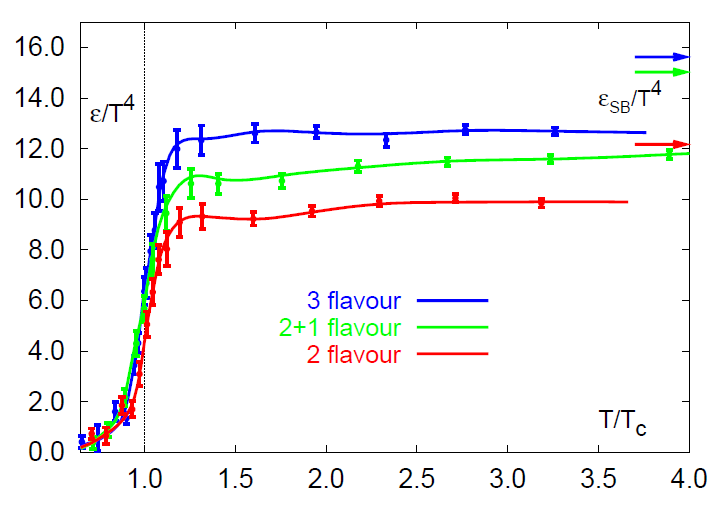
\includegraphics [width = 0.55\linewidth] {Intro/EnergyDensity_QCD.png}
		\caption{Результаты решеточной КХД [1] для плотности энергии / T4 как функции температуры, масштабированной критической температурой Tc. Обратите внимание на стрелки справа, указывающие значения предела Стефана-Больцмана.}
		\label{img:EnergyDensityQCD}  
	\end{figure}
	
	
	Схематическое изображение фазовой диаграммы ядерной материи в приближении нулевых масс верхнего и нижнего кварков ($m_{u,d} = 0$) и бесконечной массы странного кварка ($m_s = \infty$) представлено на рис. \ref{img:PhaseDiagram}.
	%/* Следующий абзац из диплома Ильи */
	В области низких температур ($T\approx 0$ МэВ) и барионных плотностей $\mu\approx 900$ МэВ вещество находится в состоянии адронного газа, при котором кварки находятся в состоянии конфаймента.  При при увеличении темепратуры и/или барионной плотности вещество переходит в состояние КГП, в котором кварки и глюоны находятся в состоянии асимптотической свободы [8]. Теоретические модели позволяют получить оценки границ такого перехода. В области низких температур (ниже критической точки) предсказывается фазовый переход первого рода в то время, как в области высоких температур – кроссовер. При условии относительно низких значений температур и достаточно высоких значений барионного химического потенциала вещество переходит в состояние цветовой сверхпроводимости.
	
	% Считается, что при достаточно больших значениях барионного химического потенциала $\mu$ наблюдается фазовый переход первого рода между адронной материей и кварк-глюонной плазмой (КГП), а также трикритическая точка, ниже которой фазовый переход становится переходом второго рода.
	Ненулевые значения масс легких кварков резко меняют картину: фазовый переход второго рода, обозначенный пунктирной линией на рис. \ref{img:PhaseDiagram}, становится плавным кроссовером, а трикритическая точка соответственно становится критической точкой, обозначающей конец перехода первого рода, обнаруженный при более высоких значениях $\mu$.
	
	Переход из КГП в состояние адронного газа называют адронизацией кварк глюонной плазмы. Основными моделями адронизации КГП являются модель рекомбинации и модель фрагментации струн.
	
	\begin{figure}[] 
		\center
		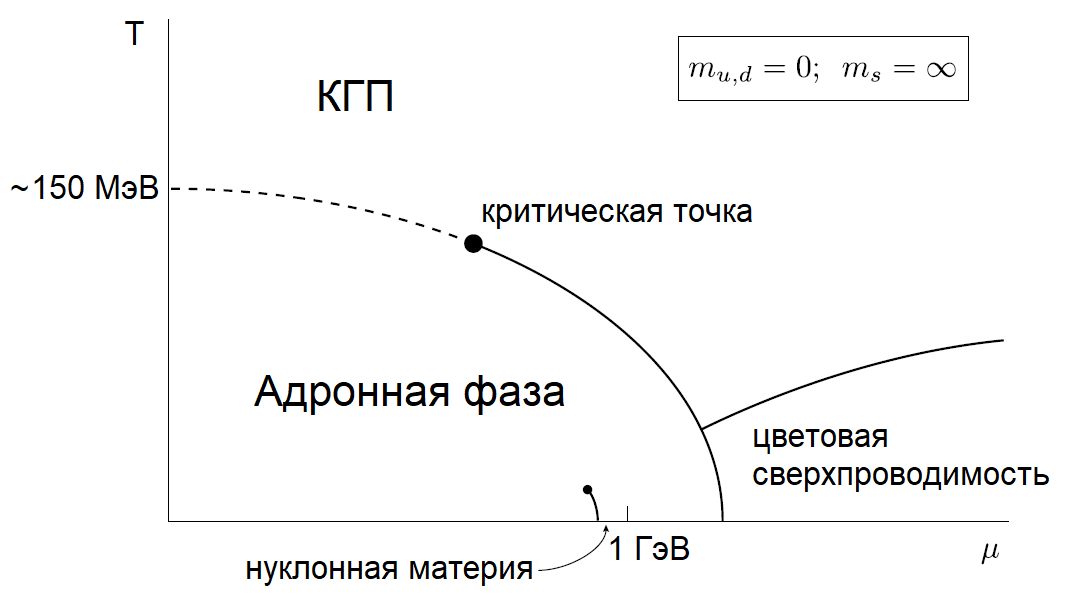
\includegraphics [width = 0.7\linewidth] {Intro/PhaseDiagram.png}
		\caption{Теоретическая фазовая диаграмма ядерной материи для двух безмассовых кварков в зависимости от температуры T и барионного химического потенциала}
		\label{img:PhaseDiagram}  
	\end{figure}
	
	
	Температура перехода соответствует плотности энергии $\epsilon = 1$ ГэВ/фм$^3$, что почти на порядок превышает плотность ядерного вещества $\epsilon_0 = 0.15$ ГэВ/фм$^3$[1407.5003]. Температуры и давления, необходимые для образования кварк-глюонной материи, достигаются в столкновениях тяжелых релятивистских ионоов.
	
	Исследованию КГП в релятивистских столкновениях посвящены такие эксперименты, как PHENIX и STAR (BNL), ALICE(CERN), CBM(JSI), MPD(NICA) и другие.
\end{comment}

\section{Эволюция столкновения тяжелых ионов}

Пространственно-временная эволюция столкновения тяжелых ионов может быть разделена на следующие фазы \cite{QGP_signatures}: 1) начальная фаза; 2) предравновесная фаза; 3) фаза термодинамического равновесия, во время которой образуется кварк-глюонная плазма; 4) фаза т.н. <<химического вымораживания>> - состояния системы частиц, когда прекращается образование новых частиц в результате неупругого рассеяния; 5) фаза т.н. <<кинетического вымораживания>> - состояния системы частиц, когда прекращаются все взаимодействия частиц и распределение частиц переходит в конечное состояние.  
Перечисленные фазы пространственно-временной эволюции показаны на рис  \ref{img:CollisionEvolution}.

Начальная фаза столкновения определяется физическими свойствами лоренцево сжатых ядер до столкновения. Непосредственно после соударения наступает предравновесная фаза. Далее в момент времени $\tau_0$ ядерная материя переходит в равновестное состояние КГП. По мере расширения, КГП остывает и при достижении критической температуры $T_c$ происходит процесс адронизации - фазовый переход в нейтральную по цвету адронную материю. Кварки и глюоны объединяются в нейтральные по цвету объекты. Некоторое время ($\sim 4$ Фм/c) ядерная материя находится в смешанной фазе, состоящей из кварков и адронов. После завершения процесса адронизации наступает фаза <<химического вымораживания>> -- устанавливается химическое равновесие и система полностью переходит в состояние адронного газа. После фазы адронного каскада наступает кинематическое равновесие (фаза <<кинетического вымораживания>>), при котором устанавливаются кинематические импульсы частицы.

Адроны, образованные в результате столкновений тяжелых ионов, несут информацию о динамике столкновения и эволюции системы сталкивающихся ионов. Распределение по поперечному импульсу и выходы этих адронов являются наблюдаемыми, по которым можно судить о характеристиках ядерной материи, образованной в результате столкновения.

%Горячая и плотная материя, образующаяся в релятивистских столкновениях тяжелых ионов, может развиваться по следующему сценарию: предравновесие, тепловое (или химическое) равновесие партонов, возможное образование КГП или смешанного состояния КГП-адронный газ, газ горячих взаимодействующих адронов и, наконец, состояние замораживания, когда образовавшиеся адроны уже не сильно взаимодействуют друг с другом. На рис. \ref{img:CollisionEvolution} показана пространственно-временная эволюция среды, возникающей при столкновениях тяжелых ионов. Поскольку рожденные адроны несут информацию о динамике столкновений и всей пространственно-временной эволюции системы от начальной до конечной стадии столкновений, точная мера распределения поперечного импульса (pT) и выхода идентифицированных адронов в зависимости от геометрии столкновения необходима для пониманиядинамики столкновений и свойств созданной материи.


\begin{figure}[] 
	\center
	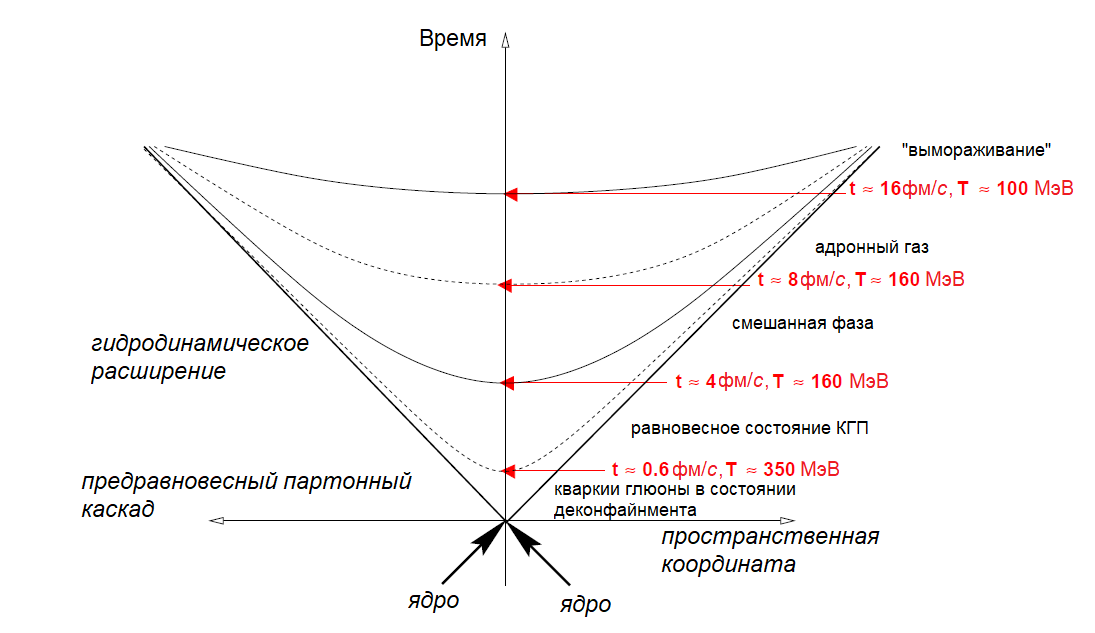
\includegraphics [width = 0.9\linewidth] {Intro/CollisionEvolution.png}
	\caption{Пространственно-временная картина ядерно-ядерного столкновения.}
	\label{img:CollisionEvolution}  
\end{figure}



\subsection{Начальная фаза столкновения} 

Описание начального состояния системы и его влияния на конечное состояние является важной задачей при изучении релятивистских столкновений. Не смотря на то, что энергии ультрарелятивистских столкновений тяжелых ионов ($\sim100$ ГэВ) на несколько порядков больше энергий связи атомных ядер ($\sim0.008$ ГэВ), детали физики ядерной структуры оказывают влияние на процесс столкновения и их необходимо учитывать при любой энергии соударения. 

Под эффектами начального состояния, также называемыми эффектами холодной ядерной материи (CNM -- Cold nuclear matter effects), понимаются все эффекты, не связанные непосредственно с образованием КГП \cite{CNM, phi_dAu, QGP_small_syst}. К эффектам CNM относят такие эффекты, как эффект Кронина \cite{Cronin, Cronin_hadrons_pp_dAu_AuAu}, многократное рассеяние частиц \cite{MPI1, MPI2}, эффекты изоспина, ядерную модификацию партонных функций  распределения \cite{PDF1, PDF2} и т.п.  


Эффекты холодной ядерной материи изучаются преимущественно на основе данных, полученных в легких системах столкновений, таких как \pal, \dau, \heau. 
С одной стороны, в легких системах столкновений присутствует лоренцево сжатое ядро, и физика холодной ядерной материи является актуальной. С другой стороны, долгое время считалось \cite{PHENIX_Nature}, что в легких системах столкновений не достигаются условия, необходимые для формирования КГП. В связи с этим, легкие системы столкновения использовались преимущественно для изучения CNM эффектов, поскольку позволяют их изучать изолированно от эффектов КГП. 

\textbf{Эффект Кронина}
К наиболее значимому эффекту холодной ядерной материи относится эффект Кронина \cite{Cronin, Cronin_hadrons_pp_dAu_AuAu, Cronin2}. 
В 1974 году Джеймс Кронин обнаружил изменение выхода частиц в нуклон ядерных столкновениях ($p$+A) по сравнению с выходом частиц в $p$+$p$ столкновениях \cite{Cronin}. 

Для описания изменения выходов частиц в $p$+A столкновениях по сравнению с $p$+$p$ столкновениями было предложено использовать фактор ядерной модификации ($R_{AB}$). Фактор ядерной модификации представляет собой отношение инвариантных спектров частиц, измеренных в $p$+A столкновениях ($1/(2\pi p_T) d^2N_{A+B}/(dp_T dy)$) и $p$+$p$ столкновениях ($1/(2\pi p_T) d^2N_{p+p}/(dp_T dy)$), нормированное на число бинарных нуклон-нуклонных столкновений, происходящих в $p$+A-столкновении (\Ncoll):

$$ R_{AB} = \frac{1}{\langle N_{coll} \rangle} \frac{d^2N_{A+B}/(dp_T dy)}{d^2N_{p+p}/(dp_T dy)}$$

Oбнаружено \cite{Cronin, Cronin_hadrons_pp_dAu_AuAu, pi0_smallSysts}, что в диапазоне малых поперечных импульсов $p_T < 2$ ГэВ/$c$ выход частиц в $p$+A столкновениях подавляется по сравнению с \pp \ столкновениями и значение фактора ядерной модификации принимает значение меньше единицы; в промежуточной области \pt \ (2 ГэВ/$c < p_T < 6 $ ГэВ/$c$) выход частиц в $p$+A столкновениях возрастает, и значение $R_{AB}$ становится больше единицы; в диапазоне больших \pt \ ($p_T > 6 $ ГэВ/$c$) выход частиц не изменяется по сравнению с выходом частиц в $p+p$ столкновениях, и $R_{AB}=1$. Увеличение выходов частиц при промежуточных значениях \pt \ принято называть пиком Кронина \cite{pi0_smallSysts}. 
В качестве примера проявления эффекта Кронина на Рисунке \ref{img:Cronin_pi0} представлены факторы ядерной модификации $\pi^0$, измеренные при энергии \sqsn=200 ГэВ экспериментом PHENIX в 2022 г \cite{pi0_smallSysts}. 

Вскоре после измерений Кронина и др. изменение выходов частиц в $p$+A столкновениях по сравнению с $p$+$p$ столкновениями было подтверждено измерениями выходов идентифицированных заряженных частиц, причем было обнаружено, что изменение выхода зависит от вида частиц \cite{Cronin2}. 

\begin{figure}[] 
	\centerfloat
	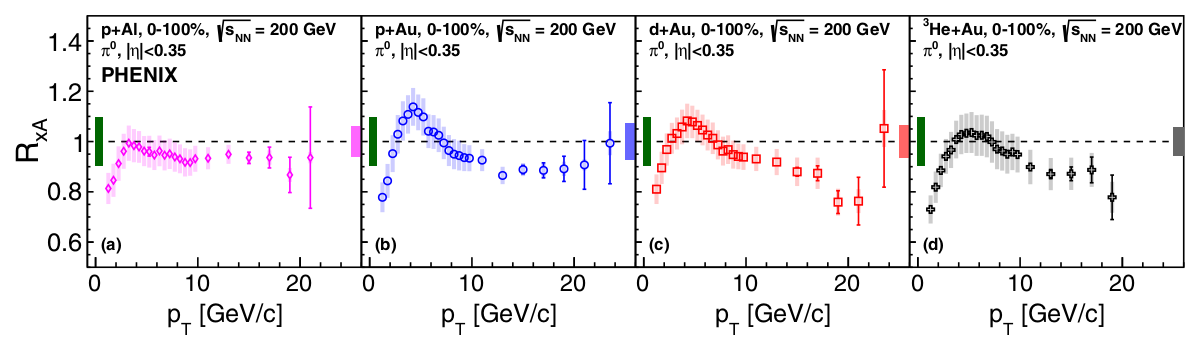
\includegraphics [width = 1\linewidth] {Intro/Cronin_pi0.png}
	\caption{Факторы ядерной модификации, полученные в неупругих столкновениях (a) $p$+Al, (b) p+Au, (c) d+Au и (d) \heau \ при \sqsn=200 ГэВ.}
	\label{img:Cronin_pi0}  
\end{figure}

Традиционное объяснение этого эффекта связано с многократным рассеянием жестких партонов от ядра-снаряда на мягких партонах ядра-мишени  \cite{Cronin_RHIC_LHC, Cronin_hadrons_pp_dAu_AuAu}.
В случае, когда функция распределения партонов $f_{b/A}(x_b, p_b^2, T)$ имеет нормированную гауссову форму, случайное упругое партонное рассеяние вызывает ее уширение по $p_T$:
$$\left< p_{b,T}^2 \right>_{pA} = \left< p_{b,T}^2 \right>_{pp} + \left< \frac{2 \mu^2 L}{\lambda_{q,g}} \right> \xi $$
где $p_{b,T}$ -- поперечный импульс партона $b$ в ядре-мишени;
$\xi = ln(1+\delta p_T^2)$. 

Значения параметров определены с помощью экспериментальных данных и составляют $\delta = 0.14$ ГэВ$^2$, $\mu^2 = 0.12$ ГэВ$^2$ и $\lambda_g = 1$ Фм.
Подход, основанный на многократном рассеянии партонов, объясняет подавление частиц при низких $p_T$ и повышение выхода частиц при промежуточных значениях $p_T$, однако не описывает зависимость эффекта Кронина от вида частиц.

В 2004 году был выдвинут иной подход, основанный на взаимодействиях в конечном, а не в начальном состоянии \cite{Cronin_Hwa}, который учитывает зависимость усиления Кронина от вида частиц.


\textbf{Потеря энергии в начальном состоянии холодной ядерной материи.}
Партоны налетающего протона претерпевают многократное рассеяние в ядре перед жестким столкновением, вследствии чего теряют энергию из-за индуцированного средой тормозного глюонного излучения \cite{InitialEnergyLoss}. Этот эффект может быть рассчитан как сдвиг доли импульса в партоных функциях распределения протона-снаряда,
$$f_{q/p}(x_a) \rightarrow f_{q/p} \left( \frac{x_a}{1-\varepsilon_{eff}} \right)$$
где $x_a$ - доля импульса протона-снаряда. Многократное излучение глюонов, $\Delta E = \sum_i \Delta E_i$, уменьшает влияние средней потери энергии, что реализуется через соотношение $\varepsilon_{eff}=0.7(\Delta E / E)$. Средняя потеря энергии зависит от передачи импульса при взаимодействии ($\mu$) между партоном и средой и длиной свободного пробега глюона ($\lambda_g$). 

\textbf{Эффект изоспина.}
Эффект изоспина оказывает влияние на наблюдаемые величины, чувствительные к аромату кварков, такие как процессы рождения фотонов или инклюзивного рождения адронов, и не оказывает существенного влияния на процессы, определяющиеся глюонами в начальном состоянии, такие как образование струй и рождение тяжелых ароматов. 

Для оценки величины эффекта изоспина используются партонные функции распределения нуклонов в ядре с атомной массой $A$ и зарядом $Z$:
$$f_{a/A}(x) = \frac{Z}{A}f_{a/p}(x)+\left(1-Z/A \right) f_{a/n}(x)$$
где $f_{a/p}(x)$ и $f_{a/n}(x)$ - партонные функции распределения протона и нейтрона соответственно. 

\textbf{Ядерная модификация партонных функций распределения.}
Партонные функции распределения (PDF -- parton distribution functions) в свободном протоне в настоящее время хорошо изучены \cite{PDF1, PDF2, PDF3}.
Однако, функции распределения партонов в нуклонах ядра отличаются от PDF в свободных нуклонах. Различие PDF в свободных и связанных партонах называется ядерной модификацией PDF. 
Определение параметров PDF в связанных нуклонах ядра проводится с помощью аппроксимации экспериментальных данных.

\textbf{Динамическое затенение.}
Последовательное когерентное рассеяние партонов-участников приводит к затенению в высших порядках наблюдаемого сечения. Данный эффект может быть учтен путем изменения доли импульса партонных функций распределения ядра-мишени:
$$x_b \rightarrow x_b \left(1+C_d  \frac{\xi^2 (A^{1⁄3}-1)}{-\hat{t}} \right)$$
где $x_b$ - доля импульса партона в ядре-мишени. Здесь $\xi ^2$ = 0,12 ГэВ$^2$ – характерный масштаб энергии многократного рассеяния. 


\subsection{Фаза столкновения} 
Cхема столкновения тяжелых ионов изображена на Рисунке \ref{img:CollisionGeometry}. Ось столкновения ядер сонаправлена оси z. Плоскость, образованную прицельным параметром (b) и осью z, называют плоскостью реакции.  
Нуклоны, испытавшие хотя бы одно неупругое столкновение, называют нуклонами-участниками. Нуклоны, которые не испытали столкновения с нуклонами другого ядра, называют нуклонами-наблюдателями.

Основными параметрами, характеризующими фазу столкновения являются прицельный параметр, центральность, количество нуклонов-участников \Npart \ и количество парных нуклон-нуклонных соударений \Ncoll.
В столкновениях релятивистских ионов прицельный параметр определяется аналогично классической механике (Рисунок \ref{img:CollisionGeometry}). Центральность столкновения характеризует степень перекрытия сталкивающихся ядер и выражается в процентах. Центральности 0\% соответствует лобовое столкновение двух ядер с максимальной степенью их перекрытия, а центральности 100\% соответсвуют наиболее переферические столкновения.
Таким образом, самым центральным столкновениям соответствуют наибольшие значения \Npart, а самым периферийным -- наименьшие.
Экспериментальное измерение центральности описано в разделе \ref{sect3:centr}. Экспериментальное определение значений $N_{part}$ и $N_{coll}$ невозможно, так как радиус сталкивающихся ядер составляет величину порядка нескольких ферми. Тем не менее, существуют модели, позволяющие оценить величины \Npart \ и \Ncoll. Одной из таких моделей является модель Глаубера \cite{Glauber}.

\begin{figure}[] 
	\centerfloat
	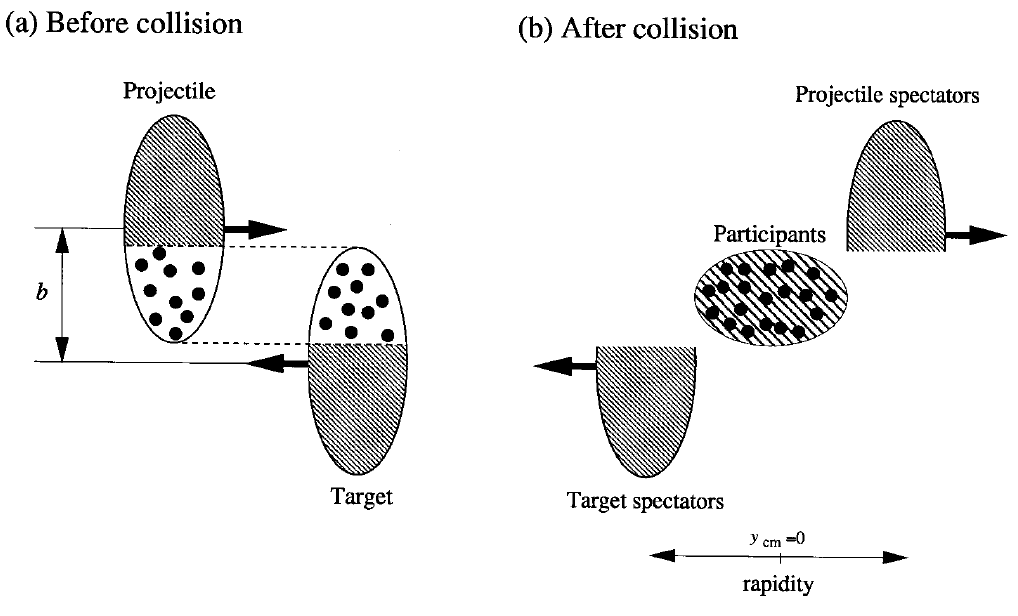
\includegraphics [width = 0.7\linewidth] {Intro/CollisionGeometry.png}
	\caption{Схематичное изображение столкновения тяжелых ионов высокой энергии с прицельным параметром b. Слева (а) показаны два сталкивающихся ядра в центре масс. Справа (б) изображена картина после столкновения -- нуклоны разделяются на участников, наблюдателей-снарядов и наблюдателей-мишеней.}
	\label{img:CollisionGeometry}  
\end{figure}

\subsubsection{Модель Глаубера}
Модель Глаубера \cite{Glauber} является полуклассической моделью столкновения релятивистских ионов, рассматривающей ядерные столкновения как множественные нуклон-нуклонные взаимодействия: нуклон налетающего ядра взаимодействует с нуклонами-мишенями при заданной плотности распределении нуклонов. Предполагается, что нуклоны движутся по прямолинейным траекториям и не отклоняются даже после столкновений, что является допустимым приближением при энергиях $\sqrt{s_{NN}} \sim 200$ ГэВ. Второе предположение состоит в том, что неупругое сечение нуклон-нуклонных взаимодействий $\sigma^{in}_{NN}$ не зависит от свойств среды и совпадает с $\sigma^{in}_{NN}$ в вакууме. Нуклоны распределены в ядре случайным образом в соответствии с распределением Вудса-Саксона. Плотность распределения нуклонов в ядре $\rho(r)$ определяется как
$$\rho(r) = \rho_0 \cdot \frac{1}{1+exp{\frac{r-R}{a}}}$$
где $R$ — радиус ядра;

$a$ — параметр поверхностной диффузии;

$\rho_0$ -- константа. 

Профиль плотности золота показан на Рисунке \ref{img:WoodSaxon}. Для иона Au параметры $R$ = 6.38 фм, $a$ = 0.54 фм и $\rho_0$ = 0.169 фм$^{-3}$. Величина неупругого нуклон-нуклонное сечения $\sigma^{in}_{NN}$ = 42 мб определена экспериментально и используется для вычисления инвариантных спектров частиц в столкновениях тяжелых ионов.

\begin{figure}[] 
	\centerfloat
	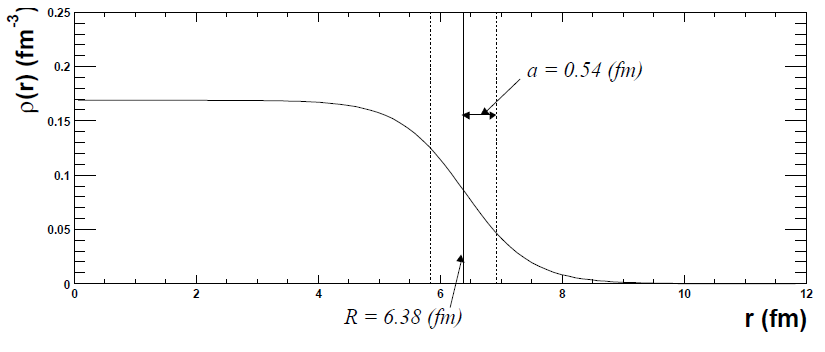
\includegraphics [width = 0.6\linewidth] {Intro/WoodSaxon.png}
	\caption{Профиль ядерной плотности Вудса-Саксона для Au.}
	\label{img:WoodSaxon}  
\end{figure}


%Сигналы от наиболее переферийных столкновений являются слишком слабыми, в результате чего такие столкновения не проходят минимальный порог срабатывания MB триггера. В эксперименте PHENIX в столкновениях, например, Сu+Au могут быть зарегистрированы только события с центральностью от 0\% до 84\%.

%что каждый интервал по центральности, выраженный в процентах от общего неупругого сечения ядро+ядро, имеет такую же вероятность, как и все остальные бины, и поэтому распределение центральности является плоским по определению. На рис. 1.3 показана зависимость энергии, депонированной в калориметрах с нулевым градусом (ZDC), от полного заряда, индуцированного в счетчиках пучка (BBC). Подробно о работе ББК и ЗДК будет рассказано в следующей главе.

%Распределение делится на перцентили вероятности равенства. ZDC измеряет энергию спектральных нейтронов, которых больше в периферийных столкновениях. И наоборот, в более центральных столкновениях образуется больше заряженных частиц, поэтому суммарный заряд, индуцированный в БВС, больше. Столкновения с исчезающим параметром соударения, т.е. с полным перекрытием, называются "наиболее центральными"; столкновения, в которых параметр соударения почти равен ядерному радиусу, т.е. практически отсутствует перекрытие, называются "наиболее периферийными". 


\subsection{Термализация}

%Дословно из Емельянова
В результате адрон-адронных взаимодействий образуются партоны двух типов: жесткие и мягкие, различающиеся по величине \pt. Жесткие партоны ($p_T \gtrsim 1.5$ ГэВ/c) не участвует в коллективных взаимодействиях и формируют вторичные адроны во фрагментационных процессах. Мягкие партоны ($p_T \lesssim 1.5$ ГэВ/c) взаимодействуют друг с другом, образуя кварк-глюонную систему.

Согласно расчетам КХД, при достижении температуры $T\approx175$ МэВ и плотности $\sim10$ ГэВ/Фм$^3$ многократные взаимодействия мягких партонов могут создать условия, достаточные для установления термодинамического равновесия и образования КГП\cite{QGP}. Последующая эволюция (расширение) системы частиц происходит по законам гидро- и термодинамики и сопровождается падением температуры системы. 
%Условия, необходимые для установления термодинамического равновесия, могут достигаться в столкновениях релятивистских тяжелых ионов, характеризующихся значениями \Npart$>10$.  

Теоретические расчеты КХД на решетке однозначно идентифицируют фазовый переход, а также позволяют определить критическую температуру фазового перехода адронной материи в КГП только в приближении нулевого барионного химического потенциала \cite{LatticeQCD_PhaseTransition1, LatticeQCD_PhaseTransition2}. 
Для экстраполяции результатов к неравновесному барионному химическому потенциалу необходимо использовать модели. Одной из наиболее удачных теоретических моделей, возникших в ранний период развития физики тяжелых ионов, является тепловая модель \cite{ThermalModel}. Основная идея тепловой модели состоит в использовании большого канонического ансамбля для описания партонной системы. 

Большой канонический ансамбль определяется как статистический ансамбль, отвечающий физической системе, способной обмениваться энергией и частицами с окружающей средой и находится с ней в тепловом равновесии.  Большой канонический ансамбль характеризуется сохранением общего количества частиц ($N$) и сохранением энергии системы ($E$). Для описания партонной системы данный формализм  большого канонического ансамбля можно расширить. Согласно тепловым моделям, рассматривающим столкновения тяжелых ионов, сохранение энергии системы $E$ расширяется до сохранения четырехимпульса системы, а сохранение числа частиц -- до сохранения заряда, барионного числа и странности \cite{ThermalModel}. 

Количество частиц в КГП не фиксировано и может быть определено в рамках статистической физики большим каноническим ансамблем для каждого типа частиц:
$$\Omega_{GC} = -kT ln(Z)$$
где $k$ – постоянная Больцмана;
 
$T$ – температура;

$Z$ -- статистическая сумма, вид которой зависит от того, подчиняется ли частица статистике Бозе-Эйнштейна или статистике Ферми-Дирака.

Множественность рождения адрона $h$ описывается следующей формулой:
$$ N_h = V\cdot n_h = \frac{V g_h}{(2 \pi \hbar)^2} \int f_h(p)d^3p$$
где $n_h$ – число степеней свободы;

$g_h=2J_h+1$ – фактор спинового вырождения;

$f_h(p)$ -- функция распределения импульса;

\begin{comment}
	При взаимодействии частиц в адронном газе неизменными схраняющимися величинами являются барионное число, заряд и странность. Химический потенциал представляет собой линейную комбинацию трех потенциалов:
	
	$$\mu_h=h_B B_h + \mu_Q Q_h + \mu_S S_h$$
	где $B_h$ – барионное число адрона $h$, 
	$Q_h$- зарядовое число адрона $h$, 
	$S$ -  странность адрона $h$.
	Данная формула может быть расширена добавлением потоенциалов для C (charm) и B (bottomness) кварков.
\end{comment}

Термодинамический подход описывает выходы частиц в столкновениях тяжелых ионов (см. Рисунки \ref{img:RatiosThermal1} и \ref{img:RatiosThermal2}), что свидетельствует о наличии фазы термализации в столкновении. 


% Карш [33] и Браун-Мунцингер [34] содержат прекрасные обзоры, посвященные решеточным результатам и тепловой модели, соответственно.
\begin{figure}[] 
	\centerfloat
	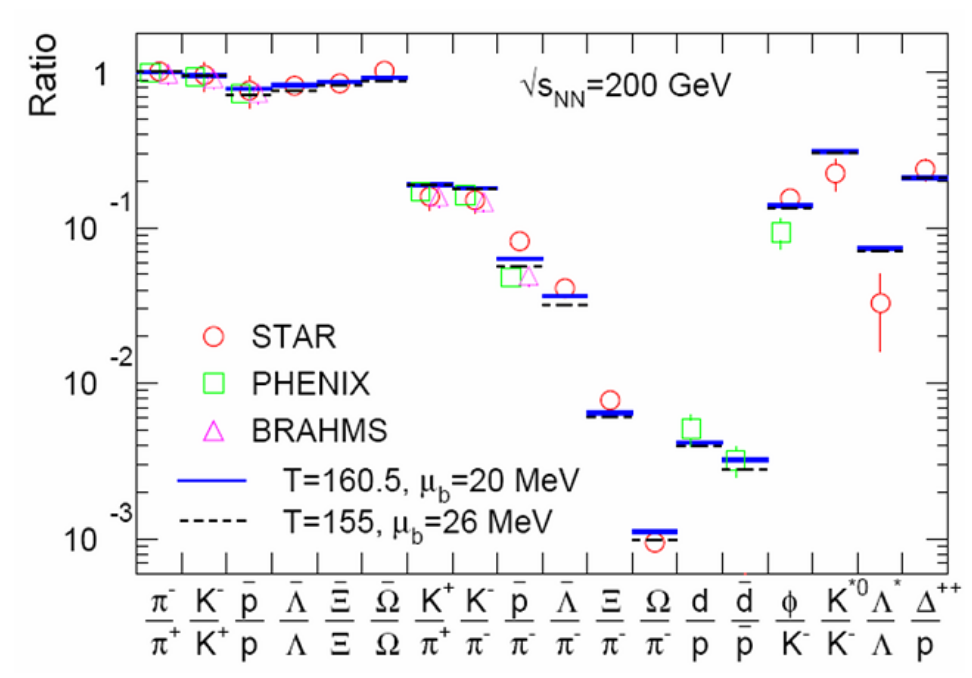
\includegraphics [width = 0.7\linewidth]
	{Intro/RatiosThermalModel1.png}
	\caption{Сравнение эксперементально измеренных отношений выходов частиц с теоретическими расчетами. В теоретической модели был использован параметр подавления странности $\gamma_s = 1$.}
	\label{img:RatiosThermal1}  
\end{figure}

\begin{figure}[] 
	\centerfloat
	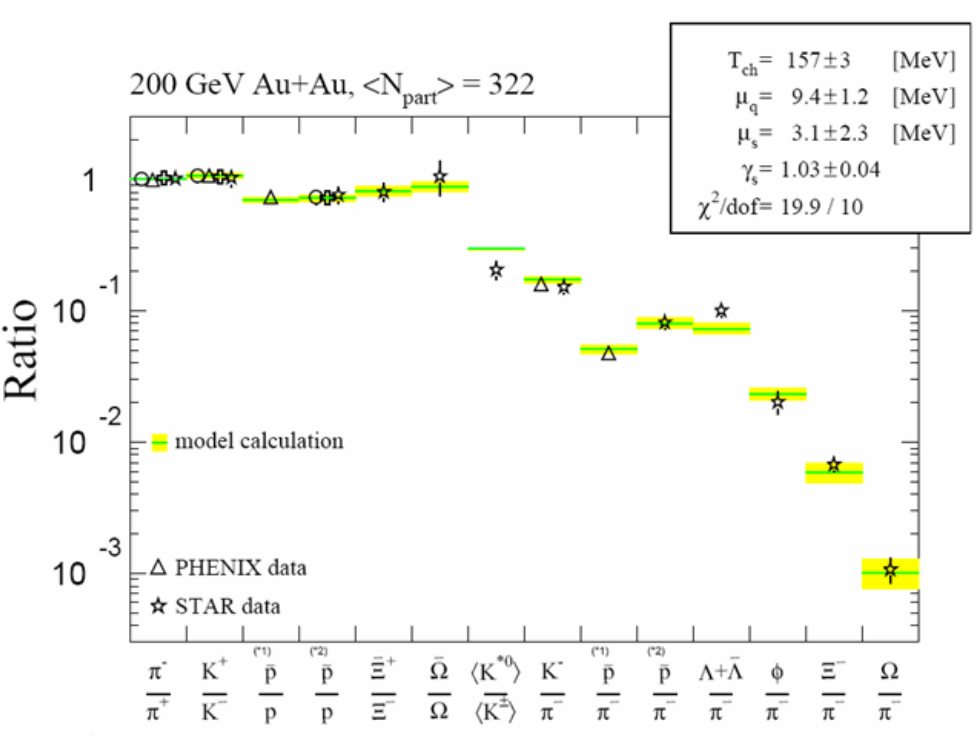
\includegraphics [width = 0.7\linewidth]
	{Intro/RatiosThermalModel2.png}
	\caption{Сравнение эксперементально измеренных отношений выходов частиц с теоретическими расчетами. В данной  теоретической модели параметр подавления странности является свободным и его значение оказывается равным $\gamma_s = 1.03 \pm 0.04$.}
	\label{img:RatiosThermal2}
\end{figure}

\begin{figure}[] 
	\centerfloat
	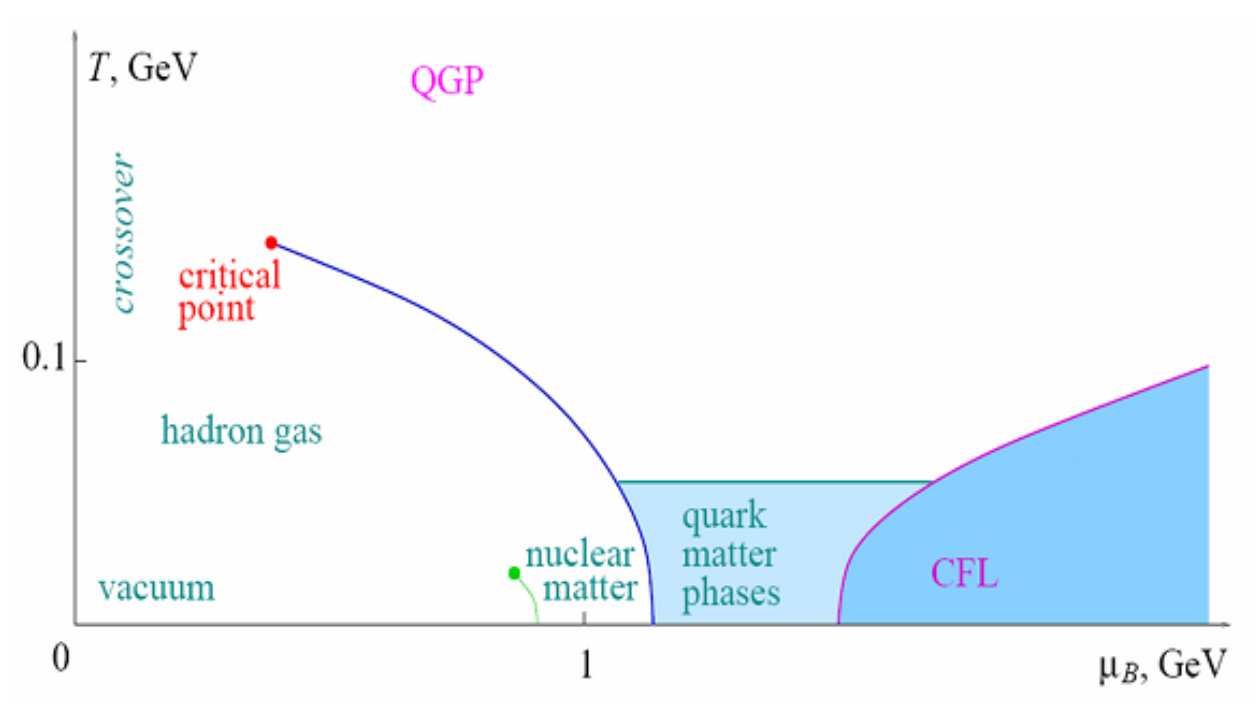
\includegraphics [width = 0.7\linewidth]
	{Intro/PhaseDiagram_Ron.png}
	\caption{Фазовая диаграмма ядерной материи.}
	\label{img:PhaseDiagram_Ron}  
\end{figure}

Основными свободными параметрами тепловых моделей при описании экспериментальных данных являются температура химического вымораживания ($T$), барионный химический потенциал ($\mu_B$) и степень уравновешивания странности. В КГП массы кварков уменьшаются до их хиггсовских масс \cite{ThermalStrangeness}; см. Рисунок \ref{img:HiggsMasses}. Хиггсовская масса странного кварка составляет $\sim$150 МэВ, что соответствует значению критической температуры. Таким образом, согласно тепловым моделям странные кварки образовываются и термализовываются так же, как и более легкие $u$ и $d$ кварки, что согласуется с результатами, представленными на Рисунке \ref{img:RatiosThermal1} и \ref{img:RatiosThermal2}. Другим подтверждением механизма образования странного кварка в тепловых моделях являются величины отношений $K/\pi$, измеренные в зависимости от \Npart (Рисунок \ref{img:Kpi_Npart}). При значениях \Npart \ $\lesssim 100$ наблюдается рост значений $K/\pi$, однако при \Npart \ $\gtrsim 100$ величины $K/\pi$ выходят на плато. Данное наблюдение свидетельствует о том, что с увеличением числа частиц в системе уравновешивание странности увеличивается, пока не достигнет определенного значения, при котором странность уравновешивается. 
\begin{figure}[] 
	\centerfloat
	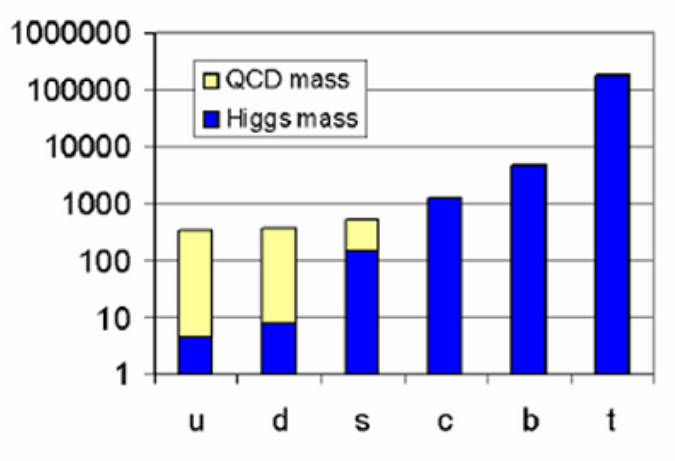
\includegraphics [width = 0.7\linewidth]
	{Intro/HiggsMasses.png}
	\caption{Вклад КХД и Хиггса в массы кварков \cite{ThermalStrangeness}.}
	\label{img:HiggsMasses}  
\end{figure}

\begin{figure}[] 
	\centerfloat
	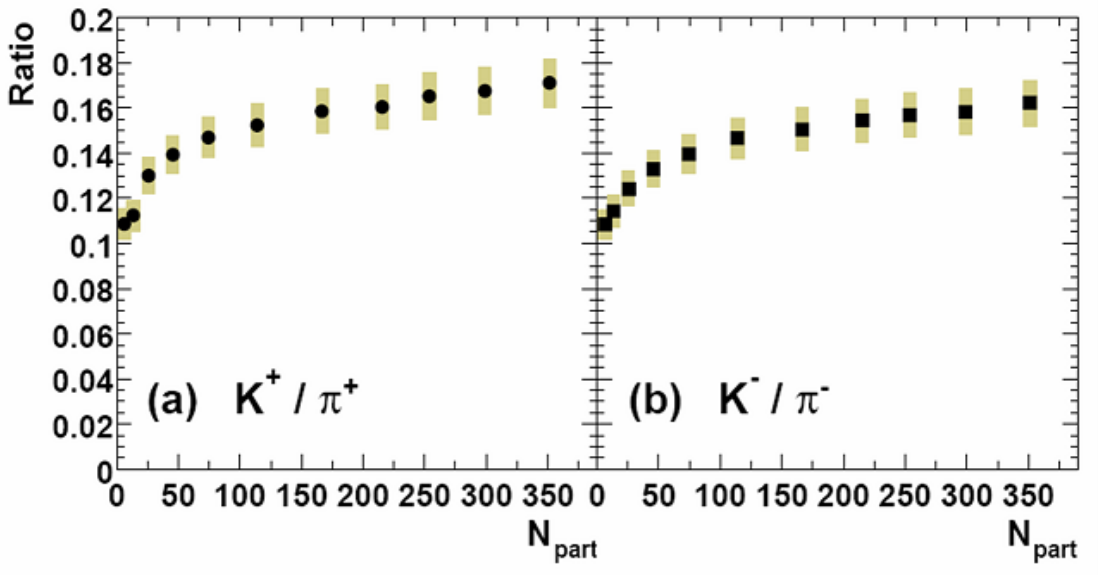
\includegraphics [width = 0.7\linewidth]
	{Intro/Kpi_Npart.png}
	\caption{Зависимость отношений $K/\pi$ от \Npart.}
	\label{img:Kpi_Npart}
\end{figure}

\begin{comment}
Для полного обоснования идеи насыщения странности с ростом \Npart \ необходимо также рассмотреть частицы со значениями странности $S=2,3$. На рис. \ref{img:StrangenessEquilibrium} показан параметр уравновешенности странности $\gamma_s$ в зависимости от числа частиц в системе. параметр $\gamma_s$ как функция от \Npart.

\begin{figure}[] 
	\centerfloat
	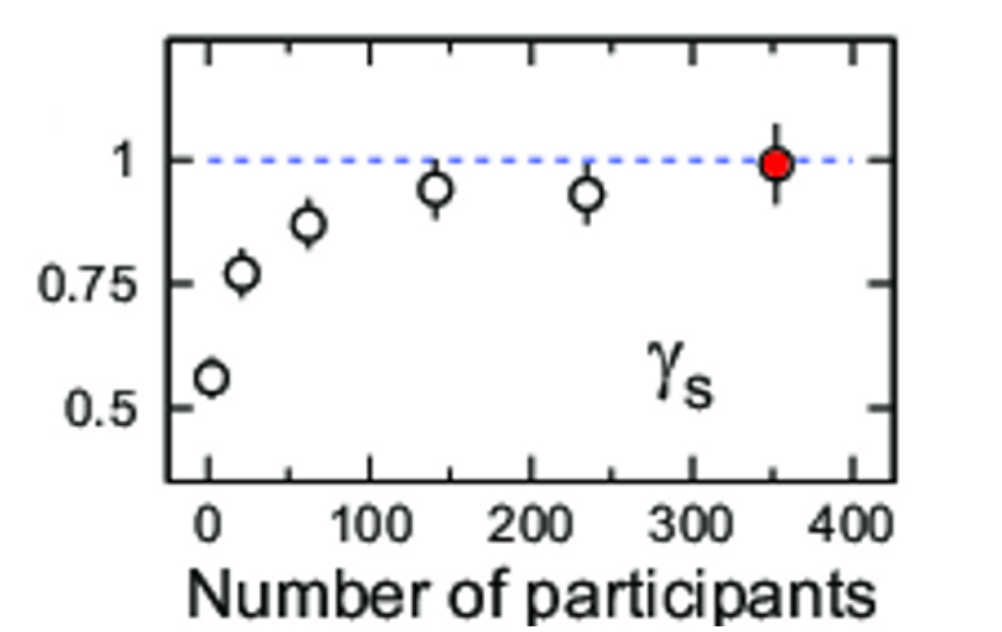
\includegraphics [width = 0.7\linewidth]
	{Intro/StrangenessEquilibrium.png}
	\caption{Параметр уравновешивания странности $\gamma_S$ как функция от \Npart}
	\label{img:StrangenessEquilibrium}
\end{figure}
\end{comment}

\subsection{Фаза гидродинамического расширения} \label{ch1/hydro}
В 1950-х годах для описания процессов множественного рождения частиц при столкновениях быстрых частиц была предложена гидродинамическая модель \cite{HydroLandau}, которая и по настоящеее время остается одной из наиболее эффективных моделей для описания взаимодействия релятивистских ядер \cite{HydroPartonicCascade, Flow1, Flow2}.
Согласно гидродинамической модели, в столкновениях релятивистских тяжелых ионов на стадии образования КГП, в результате сильного взаимодействия, устанавливается статистическое равновесие, а образовавшаяся КГП рассматривается как релятивистская жидкость.
Горячая и плотная материя, образовавшаяся в результате столкновения, увеличивается в размерах за счет множественного образования частиц.
Таким образом, система достигает состояния теплового и химического равновесия, что позволяет применить статистические тепловые модели.
Затем фаза КГП сменяется смешанной фазой, в которой присутствуют одновременно КГП и адронный газ, предполагающей фазовый переход первого порядка. После завершения процесса фазового перехода первого порядка частицы (т.е. адроны) в фазе адронного газа продолжают взаимодействовать. Адронные столкновения могут привести к высокой степени теплового и химического равновесия для различных видов адронов. Адронный газ продолжает расширяться и охлаждаться. Когда средние свободные пути адронов становятся сравнимыми с общим размером системы, происходит кинетическое вымораживание.
Поскольку гидродинамические модели проявляют зависимость от количества степеней свободы системы, изучение особенностей рождения частиц в рамках моделей гидродинамики могут дать представление о том, какие типы частиц являются его составляющими: адроны или партоны \cite{Flow1, Flow2}.

\begin{comment}
Суть релятивистской гидродинамики можно кратко изложить с помощью основных уравнений \cite{Flow1}. Тензор напряжения определяется согласно следующему выражению:
\begin{equation}
	T^{\mu \nu}(x) = (\varepsilon(x)+p(x))u^{\mu}(x)u^{\nu}(x)+p(x)g^{\mu \nu}
	\label{eq:StressEnergyTensor}
\end{equation}
где $\varepsilon$ - плотность энергии, $p$ - давление, $u^{\mu}(x) = \gamma(1, v_x, v_y, v_z)$ - четырехвектор скорости, $\gamma = 1/ \sqrt{1 - v_x^2 - v_y^2 - v_z^2}$ - Лоренц-фактор, $g^{\mu \nu}$ - метрический тензор. Сохраняющиеся токи имеют вид $j_i^{\mu}(x) = n_i(x)u^{\mu}(x)$, где $n_i(x)$ - плотности чисел сохраняющихся величин (обычно заряда, барионного числа и странности). 

\begin{equation}
	\partial_{\mu}T^{\mu \nu}(x) = 0; \partial_{\mu}j^{\mu}_i(x) = 0
	\label{eq:HydronergyConvLaw}
\end{equation}

Законы сохранения \ref{eq:HydronergyConvLaw} определяют уравнения движения.  Количеству сохраняемых величин $k$ соответствует $2~+~k$ уравнений движения, содержащих $3~+~k$ неизвестных. Таким образом, для определения всех неизвестных необходимо еще одно уравнение. Недостающим уравнением является уравнение состояния, которое связывает плотность энергии, давление и плотность чисел сохраняемых величин. 
Уравнение состояния не может быть определено из первоначальных принципов и составляется с помощью расчетов КХД на решетке. 
\end{comment}

Поток расширяющейся кварк-глюонной материи состоит из двух компонент: радиальной и анизотропной (эллиптической, триангулярной и т.п).
Под радиальным потоком понимается равномерное расширение системы во всех направлениях. Экспериментальные данные подтверждают идею о том, 
что на всех этапах эволюции КГП вещество расширяется с единой для всех адронов скоростью потока [39]. Инвариантные спектры по поперечной массе ($m_T$), измеренные для мягких адронов ($p_T<2$ ГэВ/$c$), пропорциональны $e^{m_T/T}$:

\begin{equation}
	\frac{d^2N}{m_Tdm_T} \sim e^{-m_T/T}
	\label{eq:InvSlopeRon}
\end{equation}

В случае чисто теплового движения все частицы (независимо от их массы) двигаются с одной и той же средней кинетической энергией, определяемой температурой, т.е.
$$\langle E_{kin} \rangle \sim T_{thermal}$$
С другой стороны, в случае абсолютного коллективного движения все частицы двигаются с одинаковой поперечной скоростью \ut \ и, следовательно, их кинетическая энергиях пропорциональна массе:
$$\langle E_{collective} \rangle \sim m_0 \langle u_T ^2 \rangle $$
В предположении полной независимости теплового и коллективного движения частицы полная кинетическая энергия будет равна:
$$ \langle E_{kin} \rangle = \langle E_{thermal} \rangle + \langle E_{collective} \rangle = T_{thermal}+ m_0 \langle u_T ^2 \rangle $$
где $ \langle u_T ^2 \rangle$ - средняя коллективная поперечная скорость для частиц всех типов. 

%dthesis_CH_PHENIX

\begin{comment}
/* Collective expansion */
Наиболее удачное описание различных параметров наклона и изменения формы, наблюдаемых в $m_T$-спектрах в $A+A$-столкновениях, дает термодинамическая модель при учете коллективного движения частиц. %включающая общее поперечное расширяющееся поле скоростей вместе с умеренной температурой термализованной системы. 
Качественно зависимость параметров обратного наклона спектра от массы адрона в рамках данной модели можно следующим образом [12]. В случае исключительно теплового движения все частицы (независимо от их массы) двигались бы с одной и той же средней кинетической энергией, определяемой температурой, т. е.

\begin{equation}
	\left< E_{kin} \right>  \sim T_{thermal} 
\end{equation}

С другой стороны, при исключительно коллективном движении все частицы двигались бы с одинаковой скоростью $\beta_T$ и, следовательно, средняя кинетическая энергия возрастала бы пропорционально их массе $m_0$, так как

\begin{equation}
	\left< E_{collective} \right>  \sim \frac{m_0\beta_T^2}{2}
\end{equation}

В предположении полной независимости теплового и коллективного движения частиц кинетическая энергия частиц будет опеределяться суммой $\left< E_{thermal} \right> + \left< E_{collective} \right>$, проявляя зависимость от массы адрона $m_0$:

\begin{equation}
	\begin{split}
		\left< E_{kin} \right> = \left< E_{thermal} \right> + \left< E_{collective} \right> = T_{thermal} + \frac{m_0 \left< \beta_T \right>^2}{2} 
	\end{split}
\end{equation}

где $\left< \beta_T \right>$ — усредненная скорость коллективного движения для всех видов частиц. Параметр обратного наклона $T_0$ пропорционален средней поперечной кинетической энергии и определяется как

\begin{equation}
	T_0 \sim T_{thermal} + m_0 \cdot \left< \beta_T \right>^2
\end{equation}


Кроме того, из-за этой зависимости от скорости для более тяжелой системы столкновений, в которой предположительно более сильный коллективный поперечный поток, ожидается, что значение $T_0$ будет больше. Таким образом, приведенные выше наблюдения качественно согласуются с гипотезой о поперечном гидродинамическом течении, возникающем при столкновениях тяжелых ионов.

Количественно феноменологическая гидродинамическая модель, предложенная Schnedermann et. др. [13] можно применить к спектрам одиночных частиц для извлечения поперечной скорости и температуры при замораживании. В этой модели, называемой моделью «взрывной волны», эффекты коллективного расширения включаются в спектры поперечных масс следующим образом:

\begin{linenomath}
	\begin{equation}
		\frac{d \sigma}{m_T dm_T} \sim \int_0^R r dr \cdot m_T 
		I_0 \left(\frac{p_T sinh(\rho)}{T_{fo}}\right) K_1 \left(\frac{m_T cosh(\rho)}{T_{fo}} \right)
	\end{equation}
\end{linenomath}
где $I_0$ и $K_1$ представляют собой модифицированные функции Бесселя, где $\rho$ представляет собой поперечное усиление, которое зависит от радиального положения в соответствии с $\rho = tanh^{-1} \beta_r(r)$. Детали этого выражения описаны в Приложении A.2. Здесь $T_{fo}$ - температура замерзания, $R$ - максимальный радиус расширяющегося источника при замораживании. Профиль поперечной скорости $\beta_r(r)$ параметризуется как $\beta_r(r) = \beta_T(r/R)^n$ с поверхностной скоростью $\beta_T$. Мы можем варьировать форму профиля скорости с индексом $n$, например, $n = 0,5,1,2$. Средняя поперечная скорость определяется как
\begin{linenomath}
	\begin{equation}
		\left< \beta_T \right> = \frac{\int_0^R \beta_r(r)r dr}{\int_0^R r dr} = \left(\frac{2}{2+n} \right)\beta_T
	\end{equation}
\end{linenomath}
По результатам подгонки средняя поперечная скорость не зависит от профиля скорости [14]. На рис. 1.8 показаны результаты подгонки гидродинамической моделью течения при центральных столкновениях Pb + Pb и S+S в области средней скорости [11]. Сплошные линии — спектры источника с $T_{fo}$ = 140 МэВ и $\beta_T$ = 0,6 ($\left< \beta_T \right>$ = 0.4) для Pb+Pb и источника с $T_{fo}$ = 140 МэВ и $\beta_T$ = 0,41 ($\left< \beta_T \right>$ = 0,27) для S+S. Как показано на рис. 1.8, все спектры частиц от пионов до протонов очень хорошо воспроизводятся с двумя параметрами, $T_{fo}$ и $\beta_T$.
\end{comment}

\subsection{Адронизация} \label{subsec:ch1/sec1_1}
Описание процесса адронизации представляет собой чрезвычайно сложную задачу, поскольку связанные адронные состояния непертурбативны в рамках КХД.
%В связи с этим особую важность имеют экспериментальные измерения рождения адронов в релятивистских столкновениях.
В настоящее время, для описания процессов адронизации преимущественно используется две модели: модель фрагментации \cite{FragmentationLund} и модель рекомбинации \cite{Coalescence_models}. 

%/* Fragmentation and Hadronization */
%Адронизация — это дальнодействующий процесс, включающий лишь небольшие передачи импульса. Следовательно, потоки энергии-импульса и квантовых чисел аромата на адронном уровне должны следовать потокам на партонном уровне. Результаты по инклюзивным спектрам и кратностям подтверждают эту гипотезу. Универсальный низкомасштабный $\alpha_s$ [19, 20, 21]. Теория возмущений хорошо работает вплоть до малых масштабов, $Q \sim 1$ ГэВ. Поэтому предположим, что $\alpha_s(Q^2)$ можно определить непертурбативно для всех $Q$, и использовать его при вычислении графов Фейнмана. Этот подход дает хорошее описание спектров тяжелых кварков и форм событий.
%Приведенные выше общие идеи не пытаются описать механизм образования адронов. Для этого мы пока должны прибегать к моделям. Основными современными моделями являются кластерная и струнная адронизация (рис. 2). Мы кратко опишем версии, используемые в генераторах событий HERWIG и JETSET соответственно.


\begin{comment}
	\textbf{Кластерная модель} [22]-[26]. Модель начинается с непертурбативного расщепления глюонов g → qq после партонного потока. Комбинации цвет-синглет qq имеют меньшие массы и универсальный спектр из-за свойства предконфайнмента [27, 28] ливня (рис. 3 [29]). Предполагается, что эти синглетно-цветовые комбинации образуют кластеры, которые в большинстве случаев подвергаются простому изотропному распаду на пары адронов, выбранные в соответствии с плотностью состояний с соответствующими квантовыми числами [23]. Эта модель имеет мало параметров и естественный механизм генерации поперечных импульсов и подавления рождения тяжелых частиц при адронизации. Однако у него есть проблемы с распадом очень массивных кластеров и с адекватным подавлением рождения барионов и тяжелых кварков.
	
	\textbf{Струнная модель} Эта модель основана на динамике релятивистской струны, представляющей собой цветовой поток, натянутый между исходными $q\bar{q}$. Струна создает линейный потенциал удержания и закон площадей для матричных элементов:
	$$|M(q\bar{q} \rightarrow h_1 ... h_n)|^2 \sim e^{-b A}$$
	где $A$ — заметаемая область пространства-времени (рис. 4). Струна распадается на адроны за счет образования пары $q\bar{q}$ в ее интенсивном цветовом поле. Глюоны, образующиеся в потоке партонов, вызывают «перегибы» на струне. Модель имеет дополнительные параметры для распределения поперечного импульса и подавления тяжелых частиц. У нее есть некоторые проблемы с описанием рождения барионов, но меньше, чем у кластерной модели.
	
	\textbf{Модель UCLA} [35]-[37] представляет собой вариант струнной модели JETSET, в которой приведенный выше закон площадей для матричных элементов рассматривается более серьезно и используется для определения относительных скоростей образования различных видов адронов. Это приводит к подавлению тяжелых частиц без дополнительных параметров, причем квадрат массы адрона пропорционален его площади в пространстве-времени. В настоящее время модель по-прежнему использует дополнительные параметры для $p_T$-спектров и снова имеет некоторые проблемы с описанием образования барионов.
\end{comment}

%====================== Ron ================
Долгое время единственным механизом адронизации считался механизм фрагментации, согласно которому адроны формируются в результате разрыва струн между сильновзаимодействующими партонами (см. \ref{ch1/fragmentation}).
В рамках фрагментационной модели предполагалось, что взаимодействие партонов со средой, сопровождающееся потерями энергии, будет приводить к подавлению выходов адронов. Причем ожидалось, что степень подавления выходов частиц будет независима от их типа \cite{jet_quenching}.
Согласно экспериментальным данным, выходы мезонов, состоящих из $u$ и $d$ кварков, действительно подавляются во всех дисапазонах по \pt \ в столкновениях релятивистских тяжелых ионов, причем степень подавления мезонов совпадает в пределах систематических погрешностей измерений \cite{pi0Eta_CuAu, pi0Eta_UU}. 
Однако подавления выходов странных частиц обнаружено не было \cite{QGP_signatures, phi_dAu}, а выходы протонов в диапазоне средних \pt \ (2 Гэв/$c < p_T < 4$ ГэВ/$c$) наоборот оказались увеличенными в ядро-ядерных столкновениях по сравнению с $p+p$ столкновениями  \cite{BaryonPuzzleHeavy, PPG026}.
На Рисунке \ref{img:Rcp_AuAu} представлены ядерные модификации $\phi$ и $\pi$-мезонов по сравнению с ядерной модификацией протонов, измеренные в столкновениях Au+Au при \sqsn=200 ГэВ.

Увеличение выходов протонов в диапазоне средних \pt, обнаруженное экспериментом PHENIX в 2013г, получило название <<барионная аномалия>> \cite{BaryonPuzzleVelkovska, BaryonPuzzle2002}. В попытке объяснить полученные данные Хва и Янг выдвинули модель кварковой рекомбинации \cite{Recombination2}. Модель рекомбинации основывается на предположении, что связное адронное состояние образуется путем объединения кварков, находящихся <<близко>> в фазовом пространстве. <<Близость>> в фазовом пространсте определяется радиусом рекомбинации, являющимся одним из основных параметров  модели.

\begin{figure}[] 
	\centering
	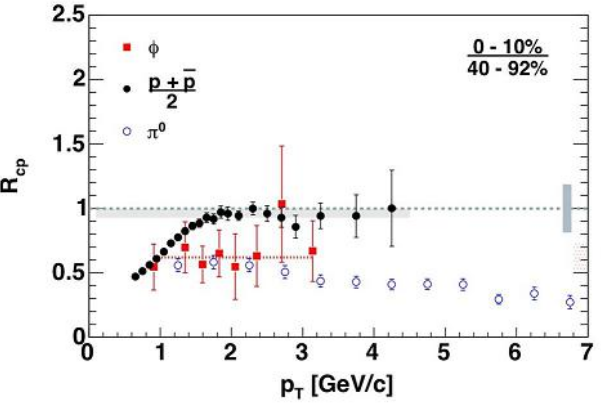
\includegraphics [width = 0.6\linewidth] {Intro/Rcp_AuAu.png}
	\caption{Ядерная модификация, измеренная для различных адронов в Au+Au столкновениях.}
	\label{img:Rcp_AuAu}  
\end{figure}


Следует отметить, что наблюдаемое отсутствие подавления протонов могло быть вызвано большей массой протонов по сравнению с мезонами. В результате радиального потока частицы движутся с одинаковыми скоростями, при этом протоны, будучи более массивными, приобритают больший импульс. Однако, как видно из Рисунка \ref{img:Rcp_AuAu}, даже мезоны с массой, равной массе протона, например, такие как $\varphi$-мезон, подавляются, что свидетельствует в пользу рекомбинационных моделей, а не зависимости подавления частиц от их массы \cite{Recombination1, Recombination2}.

В настоящее время предполагается, что рекомбинационные процессы преобладают в области $p_T \lesssim 2$ ГэВ/$c$, в то время как при $p_T \gtrsim 4$ ГэВ/$c$ преобладают процессы фрагментации. В диапазоне промежуточных поперечных импульсов (2 ГэВ/$c \lesssim p_T \lesssim $ 4 ГэВ/$c$) процессы фрагментации и рекомбинации являются конкурирующими.

\subsubsection{Модель фрагментации} \label{ch1/fragmentation}
%/* Lund fragmentation */
Фрагментационные модели основаны на принципе конфайнмента и преимущественно применяются для описания процесса адронизации жестко рассеянного партона в элементарных столкновениях. 
%Потенциал сильного взаимодействия рамках КХД имеет следующий вид:
%
%где $\alpha_s \approx 1$ - константа сильного взаимодействия, а коэффициент $\kappa ~ 1$ ГэВ/c. Наличие линейного члена было впервые установлено с помощью адронной спектроскопии, а позже подтверждено расчетами КХД на решетке. На больших расстояниях ($r > 1$ фм) доминирует линейный член. В модели фрагментации только этот член используется для описания распада массивной qq-системы на несколько менее массовых. Тогда полное цветовое поле можно аппроксимировать одномерной струной, натянутой прямо между q и q, рис. 1. Эту струну можно рассматривать как параметризующую центр цилиндрической области одинаковой ширины по всей ее длине, так что продольные и поперечные степени свободы почти полностью развязаны.
Конфайнмент принято рассматривать \cite{FragmentationLund} как проявление линейного члена в потенциале сильного взаимодействия между кварком и антикварком ($q$, $\bar{q}$) в общем цветовом синглетном состоянии:
$$ V_{QCD}(r) \approx -\frac{4}{3} \frac{\alpha_s}{r} +\kappa \cdot r$$
где $r$ — расстояние между кварком и антикварком;

$\alpha_{s}$ — константа сильного взаимодействия;

коэффициент $\kappa \approx 1$ ГэВ/фм.

Наличие линейного члена потенциала взаимодействия было впервые обнаружено с помощью адронной спектроскопии, а позже подтверждено расчетами КХД на решетке. 

Цветовое поле, возникающее при сильном взаимодействии двух цветовых зарядов ($q$, $\bar{q}$), можно представить в виде одномерной струны, натянутой между $q$ и $\bar{q}$, Рисунок \ref{img:Fragmentation}. 
При увеличении расстояния между $q$ и $\bar{q}$ струна растягивается, а величина потенциала $V_{QCD}(r)$ растет. Когда величина $V_{QCD}(r)$ превышает порог рождения кварк-антикварковой пары, происходит разрыв струны с дальнейшим формированием адронов.  
%Растяжение струны продолжается до тех пор, когда энергетичски более выгодным появление новой кварк-антикварковой пары, а не удлинение трубки
%При увеличении расстояния между двумя цветовыми зарядами, квакром и антикварком, вклад линейного члена $V_{QCD}$ растет. В какой-то момент становится энергетически выгодным появление новой кварк-антикварковой пары, а не удлинение трубки. В результате этого, когда кварки образуются в ускорителях частиц, вместо того, чтобы видеть отдельные кварки в детекторах, ученые видят "струи" из множества нейтральных по цвету частиц (мезонов и барионов), сгруппированных вместе. Этот процесс называется адронизацией, фрагментацией или разрывом струны.

\begin{figure}[] 
	\center
	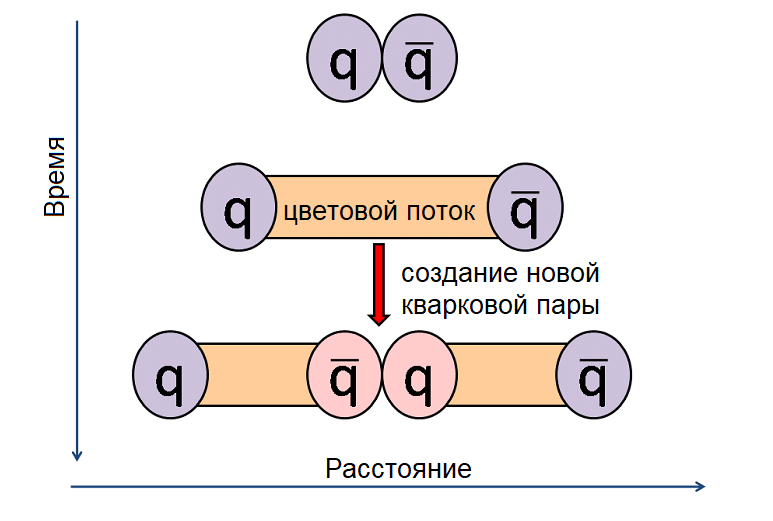
\includegraphics [width = 0.6\linewidth] {Intro/fragmentation model color}
	\caption{Схематическое изображение процесса формирование адронов согласно модели фрагментации.}
	\label{img:Fragmentation}  
\end{figure}

В рамках модели фрагментации инвариантный \pt \ спектр адронов может быть вычислен согласно следующему выражению:

\begin{equation}
	E \frac{d^3 N_h}{d^3p} = \int d\Sigma \frac{P\cdot u}{(2 \pi)^3} \sum_{\alpha}\int dz z^{-3} \omega_{\alpha}(P/z)D_{\alpha \rightarrow h}(z)
\end{equation}	
где $\Sigma$ -- гиперповерхность химического вымораживания;

$P$ -- четырехвектор импульса адрона;

$u$ -- четырехвектор скорости коллективного расширения системы;

$\omega$ -- распределение кварков в фазовом пространстве;

$\alpha$ -- партонные степени свободы;

$z$ -- доля импульса адрона $h$;

$D(z)$ -- функция фрагментации. 

Функция фрагментации не может быть вычислена аналитически и определяется исходя из соответствия экспериментальным данным.

%Таким образом, модель фрагментации основана на нескольких общих предположениях: (i) частицы в конечном состоянии возникают в результате разрыва силового поля, похожего на струну, натянутого между цветовыми зарядами, (ii) существует причинность и лоренц-инвариантность и (iii) производство частицы могут быть описаны в терминах стохастического процесса, который подчиняется предположению о насыщении.

%Другой моделью адронизации является модель фрагментации, согласно которой адроны образуются из партонных струй. Согласно рекомбинационной модели, адроны образуются в результате рекомбинации партонов, близких друг к другу в фазовом пространстве. Фрагментация и рекомбинация являются конкурирующими механизмами, но рекомбинация естественным образом увеличивает соотношение барион/мезон при промежуточных $p_T$, поэтому считается, что фрагментация преобладает при высоких значениях $p_T$, а рекомбинация — при средних значениях $p_T$.
%Полагают, что при энергии 200 ГэВ в области поперечных импульсов $1.5$  ГэВ/c $\leq p_T \leq 3$ ГэВ/c процессы рекомбинации являются доминирующими в процессе адронизации КГП, а при более высоких поперечных импульсах ($p_T\geq 6$  ГэВ/c)  доминирующими являются процессы фрагментации. В области поперечных импульсов $3$  ГэВ/c $\leq p_T \leq 6$ ГэВ/c Модель рекомбинации и модель фрагментации являются конкурирующими.

\subsubsection{Модель рекомбинации} \label{ch1/Recombination}
%/* Coalescence models for hadron Formation */
%Процесс адронизации из КГП может сильно отличает достижении термализации и образование большого количества партонов достигается термализация и не образуется масса партонов. В этом обзоре мы обсуждаем модель адронизации КГП путем слияния или рекомбинации кварков и глюонов. Обсуждаемые здесь модели успешно описывают многие существенные особенности образования адронов в столкновениях тяжелых ионов.
Согласно модели рекомбинации (коалесценции)\cite{Recombination1, Recombination2}, адронизация КГП происходит в результате объединения кварков, находящихся в фазовом пространстве $(x, p)$ на расстоянии меньше радиуса рекомбинации $(\Delta_x, \Delta_p)$. Величины $\Delta_x, \Delta_p$, связанные соотношением неопределенностей $\Delta_p \cdot \Delta_x \approx 1$, являются параметрами рекомбинационной модели и определяются исходя из соответствия экспериментальным данным. Процесс образования адронов путем рекомбинации схематически изображен на Рисунке \ref{img:Recombination}.

\begin{figure}[] 
	\center
	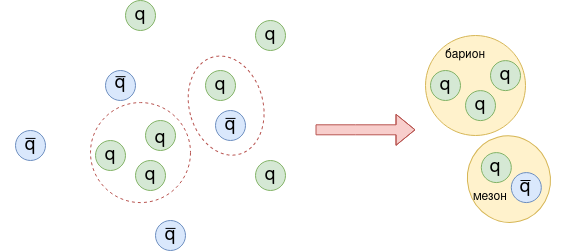
\includegraphics [width = 0.8\linewidth] {Intro/Recombination}
	\caption{Схематическое изображение процесса формирование адронов согласно модели рекомбинации. }
	\label{img:Recombination}  
\end{figure}

\begin{comment}
	Количество мезонов, имеющих определенный импульс P может быть вычислено согласно следующей формуле
	$$\frac{dN_M}{d^3 P}=\sum_{a,b}\int \frac{d^3 R}{2\pi^3} \frac{d^3 q d^3 r}{2\pi^3}  W_{ab}(R-\frac{r}{2},\frac{P}{2}-q;R+\frac{r}{2},\frac{P}{2}+q) \Phi_M (r,q) $$
	Где индекс $M$ обозначает мезон, а индексы $a$ и $b$ обозначают коалесцирующие валентные кварки. $W_{ab}$ и $\Phi_M$ – функции Вигнера для партонов и мезона соответственно, $P$ и $R$ – импульс и координата мезона, $q$ и $r$ – доли импульса, которые несут кварки, и координаты кварков. Суммирование производится по всем возможным комбинациям 
\end{comment}

Количество адронов $N_n$, содержащих $n$ кварков/акнтикарков, имеющих координаты $x_i$ и импульсы $p_i$  может быть вычислено согласно формуле \cite{Coalescence_models, Recombination1, Recombination2}:
$$ N_n=g\int \prod_{i=1}^n p_i d\sigma_i  \frac{d^3 p_i}{(2\pi)^3 E_i }  f_{q,i} (x_i,p_i ) f_n(x_1,…,x_n;p_1,…,p_n ) $$

$x_i$, $p_i$ -- координаты и компоненты трехмерных векторов импульса кварков;
 
$g$ -- спин-цветовой статистический множитель;

$f_q (x,p)$ -- функция распределения кварков. 

В качется примера значений спин-цветового статистического множитя можно привести значения $g$, рассчитанные для $\pi$ и $K$, $\rho$, $K^*$ мезонов, протонов ($p$) и антипротонов (\aprot): $g_\pi=g_K=1/36$, $g_p~=~g_{\bar{p}}~=~1/108$, $g_\rho~=~g_{K^*}~=~1/12$.
Функция распределения кварков удовлетворяет условию нормировки: 
$$\int p\cdot d\sigma \frac{d^3 p}{(2\pi)^3 E} f_q(x,p)=N_q$$
где $N_q$ -- общее количество кварков в системе.
Функции вероятности образования мезона ($f_M$) и бариона ($f_B$) путем рекомбинации могут быть найдены следующим образом \cite{Recombination1, Recombination2}:
%$$f_M (x_1,x_2;p_1,p_2 )= exp{\frac{(x_1-x_2 )^2}{2\Delta_{x^2}}} \cdot exp{\frac{(p_1-p_2 )^2-(m_1-m_2 )^2}{2\Delta_{p^2} }}$$
$$f_M (x_1,x_2;p_1,p_2 )=\frac{9 \pi}{2\Delta_{x}^3 \Delta_{p}^3} \Theta \left( \Delta_{x}^2 - (x_1 - x_2)^2  \right) \times$$
$$ \Theta \left( \Delta_{p}^2 - (p_1 - p_2)^2  + \frac{1}{4}(m_1 - m_2)^2 \right) $$


$$f_B(x_1, x_2, x_3; p_1, p_2, p_3) = \frac{9 \pi}{2\Delta_{x}^3 \Delta_{p}^3} 
\Theta \left( \Delta_{x}^2 - \frac{1}{2} (x_1 - x_2)^2\right) \times $$
$$\Theta \left( \Delta_{p}^2 - \frac{1}{2} (p_1 - p_2)^2\right) \frac{9 \pi}{2\Delta_{x}^3 \Delta_{p}^3}\times
\Theta \left( \Delta_{x}^2 - \frac{1}{6} (x_1 + x_2 - 2 x_3)^2\right) \times $$
$$\Theta \left( \Delta_{p}^2 - \frac{1}{6} \left[ (p_1 + p_2 - 2 p_3)^2 - (m_1 + m_2 -2 m_3)^2 \right] \right) $$

где $\Theta$ -- функция Хевисайда;

$m_i$, $x_i$, $p_i$ -- массы, координаты и компоненты трехмерных векторов импульса кварков;


В приведенном выражении для $f_B$ использовано приближение, согласно которому радиусы рекомбинации пространства и импульса одинаковы для трех кварков, формирующих барион. Нормировка функции $f_B$ аналогична нормировке функции вероятности коалесценции мезонов $f_M$ и составляет $(2\pi)^6$ после интегрирования по координатам и импульсам. 

Импульс адрона, образующегося в процессе рекомбинации, складывается из суммы импульсов кварков, его составляющих. Таким образом, инвариантный \pt \ спектр барионов, состоящих из трех кварков, смещается в сторону больших \pT \ по сравнению с инвариантным \pT \ спектром мезонов, состоящих из двух кварков, что приводит к увеличению выхода барионов по сравнению с выходами мезонов в области поперечных импульсов 2 ГэВ/$c$ $\lesssim$ \pT $\lesssim$ 4 ГэВ/$c$. 

Заметим, что модель рекомбинации основана на предположении о доминировании валентных кварков, т.е. низшие фоковские состояния являются наиболее важными. 

Модель рекоминации реализована в пакете AMPT в версии с плавлением струн \cite{AMPT} (см. раздел \ref{sec:PYTHIA}). 

%/* Coalescence models for hadron Formation */
%Только модели коалесценции выдержали испытания, наложенные внушительным объемом данных, полученных после первоначального открытия барионного усиления. Они особенно привлекательны, потому что они, кажется, обеспечивают естественное объяснение масштабирования числа валентных кварков, которое наблюдалось в измерениях v2. Они также связывают адронные наблюдаемые с доадронной стадией взаимодействия кварков и глюонов. Таким образом, они касаются центральных вопросов программы физики тяжелых ионов: деконфайнмента и восстановления киральной симметрии.

\subsubsection{Сравнение моделей рекомбинации и фрагментации}
Ниже приведены основные различия моделей фрагментации и рекомбинации. 

Фрагментация:
\begin{itemize}[]
	\item Инклюзивный процесс;
	\item Медленное убывание инвариантных \pt \ спектров (степенной закон);
	\item Импульс образованных адронов меньше импульсов партонов, участвовавших в процессе фрагментации;
	\item Количество образующихся мезонов $N_M$ значительно превосходит количество образующихся барионов $N_B$: $N_M \ll N_B$.
\end{itemize}

Рекомбинация:
\begin{itemize}[]
	\item Эксклюзивный процесс;
	\item Более быстрое убывание инвариантных \pt \ спектров (экспоненциальное);
	\item Импульс образованных адронов превосходит импульсы партонов, участвовавших в процессе рекомбинации;
	%\item Образуется примерно равное количество мезонов и барионов $N_M \approx N_B$.
	
\end{itemize}

\begin{comment}
	Процесс фрагментации является инклюзивным, поскольку любой жесткий партон ($p_T > 5$) может фрагментировать с образованием новых адронов, тогда как для рекомбинации необходимо, чтобы они находились в на расстоянии в фазовом пространстве меньшем, чем радиус рекомбинации. 
	Инвариантный \pt \ спектр адронов, предсказываемый моделью фрагментации, имеет более медленный спад по сравнению с тем, что предсказывает модель рекомбинаци. Фрагментация значительно благоприятствует образованию мезонов, поскольку при фрагментации с гораздо большей вероятностью образуется кварк-антикварковая пара, чем дикварк [4]. 4]; при рекомбинации они образуются примерно в равной степени.
\end{comment}
Поскольку для рекомбинационной модели характерно более быстрое убывание инвариантных \pt \ спектров, чем  для модели фрагментации, можно ожидать, что процессы рекомбинации доминируют в области малых \pt \ ($p_T<2$ ГэВ/$c$), а процессы фрагментации -- в области больших \pt \ ($p_T>4$ ГэВ/$c$). Данное предположение подтверждается экспериментальными наблюдениями. На Рисунках \ref{img:Recombination_pi0spectra}-\ref{img:Recombination_pbar} предствалено сравнение инвариантных \pt \ спектров, измеренных экспериментом PHENIX для \pio \ (Рисунки \ref{img:Recombination_pi0spectra}, \ref{img:Recombination_pi0spectra1}), заряженных адронов (Рисунок \ref{img:Recombination_all_hadrons}) и \aprot \ (Рисунок \ref{img:Recombination_pbar}), с теоретическими расчетами, основанными на модели рекомбинации. 

На Рисунке \ref{img:Frag_vs_reco} представлено схематическое изображение инвариантного \pt \ спектра легких адронов в центральных столкновениях релятивистских тяжелых ионов.
%Процессы рекомбинации доминируют в области \pT $lesssim$ 2 ГэВ/$c$, в то время как в области \pT $gtrsim$ 2 ГэВ/$c$ преобладают процессы фрагментации. 
Импульс адрона, образовавшегося в процессе рекомбинации, определяется суммой импульсов кварков его составляющих, в то время, как импульс адрона, образовавшихся в процессе фрагментации, несет лишь долю $z$ импульса жесткого партона. Таким образом, в диапазоне промежуточных \pT \ процессы фрагментации и рекомбинации являются конкурирующими.

\begin{figure}[] 
	\center
	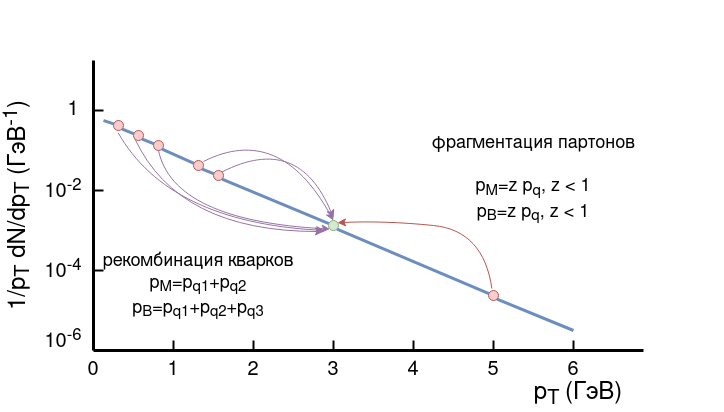
\includegraphics [width = 0.8\linewidth] {Intro/Frag_vs_Reco}
	\caption{Схематическое изображение инвариантного \pt \ спектра легких адронов в центральных столкновениях релятивистских тяжелых ионов.}
	\label{img:Frag_vs_reco}  
\end{figure}


\begin{comment}
	\subsubsection{Теоретические расчеты инвариантного спектра по поперечному импульсу}
	Полезно сравнить теоретические формулы для спектров импульсов, предсказываемых этими моделями этими моделями. Они могут быть записаны различными эквивалентными способами, здесь я привожу их в виде в [36, 57, 58]. Для фрагментации спектр импульсов имеет вид
	
	\begin{equation}
		E \frac{d^3 N_h}{d^3p} = \int d\Sigma \frac{P\cdot u}{(2 \pi)^3} \sum_{\alpha}\int dz z^{-3} \omega_{\alpha}(P/z)D_{\alpha \rightarrow h}(z)
	\end{equation}	
	
	где $\Sigma$ - гиперповерхность химического вымораживания, $P^{\mu}$ - импульс адрона, $u^{\mu}$ - скорость коллективного расширения, $\omega$ - распределение в фазовом пространстве кварков, $\alpha$ - различные степени свободы партонов, $z$ - доля импульса, $D(z)$ - функция фрагментации. Функция фрагментации не может быть вычислена аналитически, она всегда она всегда реконструируется с помощью подгонки к данным. Для рекомбинации спектр импульса имеет вид
	
	\begin{equation}
		E \frac{d^3 N^{(M)}}{d^3p} = \int d\Sigma \frac{P\cdot u}{(2 \pi)^3} \sum_{\alpha \beta}\int dx\omega_{\alpha}(xP)\bar{\omega}_{\beta}((1-x)P) |\phi^{(M)}_{\alpha, \beta}(x)|^2
	\end{equation}	
	для мезонов и 
	
	\begin{equation}
		E \frac{d^3 N^{(B)}}{d^3p} = \int d\Sigma \frac{P\cdot u}{(2 \pi)^3} \sum_{\alpha \beta \gamma}\iint dx dx' \omega_{\alpha}(xP) \omega_{\beta}(x'P) \bar{\omega}_{\gamma}((1-x-x')P) |\phi^{(B)}_{\alpha, \beta, \gamma}(x)|^2
	\end{equation}	
	для барионов.
	
	для барионов, где $x$ и $x'$ - доли импульса, а $\phi$ - волновые функции адронов. Для теплового распределения партонов распределение в фазовом пространстве имеет вид $\omega(p) = e^{p\cdot u/T}$, но при достаточно большом импульсе распределение в фазовом пространстве имеет вид степенного закона но при достаточно большом импульсе распределение в фазовом пространстве имеет вид степенного закона.
\end{comment}

\begin{figure}
	\centering
	\begin{minipage}{.47\textwidth}
		\centering
		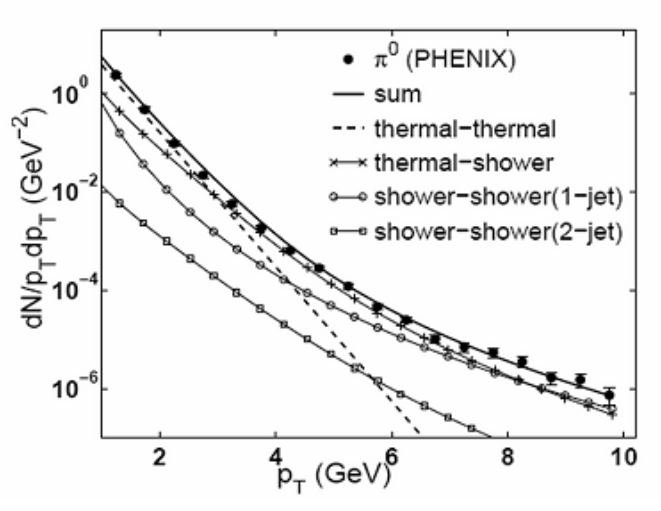
\includegraphics[width=.9\linewidth]
		{Intro/Recombination_pi0spectra}
		\captionof{figure}{Сравнение инвариантных \pt-спектров, измеренных для $\pi^0$ экспериментом PHENIX, с предсказаниями рекомбинационной модели}
		\label{img:Recombination_pi0spectra}
	\end{minipage}%
	\hfill
	\begin{minipage}{.47\textwidth}
		\centering
		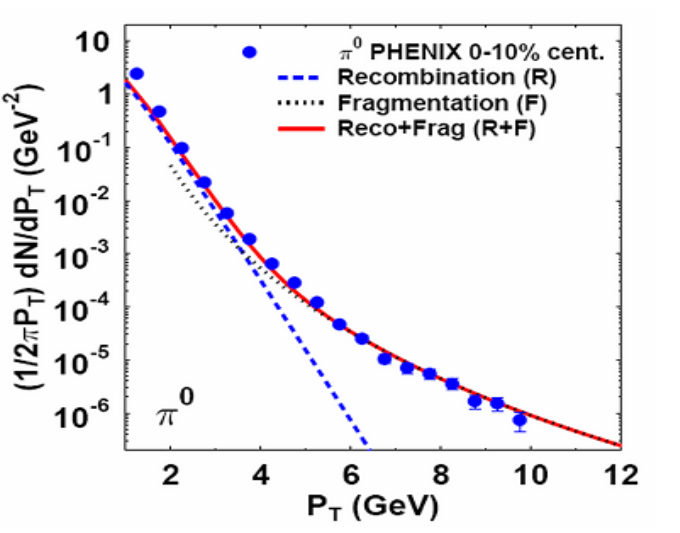
\includegraphics[width=.9\linewidth]
		{Intro/Recombination_pi0spectra1}
		\captionof{figure}{Сравнение инвариантных \pt-спектров, измеренных для $\pi^0$ экспериментом PHENIX, с предсказаниями рекомбинационной модели}
		\label{img:Recombination_pi0spectra1}
	\end{minipage}
\end{figure}


\begin{figure}
	\centering
	\begin{minipage}{.47\textwidth}
		\centering
		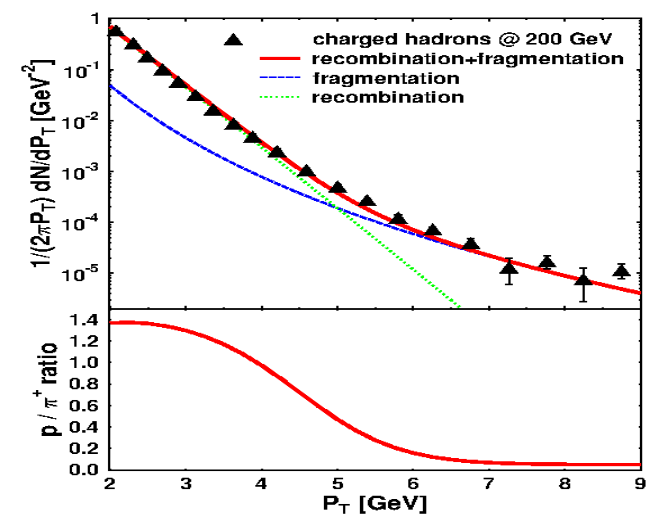
\includegraphics[width=.9\linewidth]
		{Intro/Recombination_unidentified_hadrons}
		\captionof{figure}{Сравнение инвариантных \pt-спектров, измеренных для неидентифицированных адронов экспериментом PHENIX, с предсказаниями рекомбинационной модели}
		\label{img:Recombination_all_hadrons}
	\end{minipage}%
	\hfill
	\begin{minipage}{.47\textwidth}
		\centering
		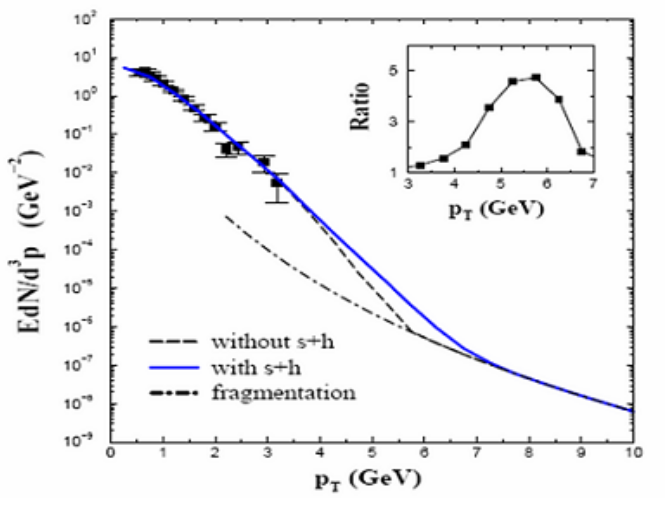
\includegraphics[width=.9\linewidth]
		{Intro/Recombination_pbar}
		\captionof{figure}{Сравнение инвариантных \pt-спектров, измеренных для $\bar{p}$ экспериментом PHENIX, с предсказаниями рекомбинационной модели}
		\label{img:Recombination_pbar}
	\end{minipage}
\end{figure}

\section{Признаки образования КГП} \label{subsec:ch1/sec1_1}
Существует ряд экспериментальных признаков, по которым можно судить о возможном образовании КГП в столкновении релятивистских тяжелых ионов. 

\textbf{Увеличенный выход барионов.}
В протон-протонных столкновениях в области поперечных импульсов $p_T \approx 3$ ГэВ/с барионов рождается в 3 раза меньше, чем мезонов \cite{Coalescence_models}. Это связано с большими массами барионов и требованием ненулевого барионного числа для образования бариона.
Однако в 2002 году экспериментом PHENIX было обнаружено, что в центральных Au+Au столкновениях при энергиях \sqsn=130 ГэВ и \sqsn=200 ГэВ \cite{BaryonPuzzleVelkovska, BaryonPuzzle2002} протоны(антипротоны) и $\pi^{\pm}$-мезоны рождаются примерно в равной пропорции (отношение выходов протонов к выходам $\pi$-мезонов ($p/\pi$) достигает значения 0.8). С уменьшением центральности столкновений различие между значениями $p/\pi$, измеренными в $p$+$p$ и Au+Au, взаимодействиях уменьшается. Единственной моделью, способной описать данную аномалию, получившую название <<барионная загадка>>, оказалась модель рекомбинации.

\textbf{Увеличенный выход странности}
-- признак образования КГП, заключающийся в увеличении выхода частиц, содержащих странный кварк \cite{StrangEnh, Strangeness_QGP}. Основными процессами рождения странного кварка является глюон-глюонное рассеяние (Рисунок \ref{img:StrangenessEnhancement} а), б), в)) и взаимодействие кварк-атикварковой пары (Рисунок \ref{img:StrangenessEnhancement} г)). В релятивистских протон-протонных столкновениях выходы адронов, содержащих тяжелые кварки, подавляются в связи с их большой массой и малой вероятностью глюон-глюонных взаимодействий. В столкновениях тяжелых релятивистских ионов, при условии формирования КГП, выход странных кварков увеличивается за счет вклада глюн-глюонного рассеяния (Рисунок \ref{img:StrangenessEnhancement} д)). В связи с этим повышенный выход странности считается одним из признаков образования КГП. 

\begin{figure}[] 
	\center
	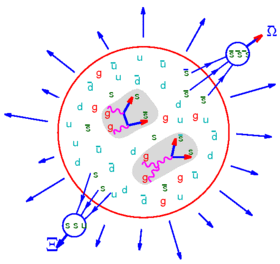
\includegraphics [width = 0.8\linewidth] {Intro/Strangeness_enhancement.png}
	\caption{Процессы, приводящие к образованию странных кварков. а), б), в) - глюон-глюонное рассеяние, г) взаимодействие кварк-антикварковой пары. д) Схема, иллюстрирующая процессы образования странных кварков в КГП.}
	\label{img:StrangenessEnhancement}  
\end{figure}
%Механизм образования странных кварков представлен на рис. \ref{img:StrangenessEnhancement}.

%Наиболее часто предлагаемые сигнатуры для возможного наблюдения КГП - это увеличение странности и появление антибарионов. В образовании пары $\bar{q}q$ при столкновении нуклонов и нуклонов высоких энергий тяжелые ароматы подавляются из-за их массы. Выход $\bar{s}s$  составляет около 0,1 $\gg$ 0,2 по сравнению с выходами $\bar{u}u$  или $\bar{d}d$. Эта ситуация может измениться при столкновениях тяжелых ионов. Если адронная материя деконфайнментируется во время столкновения тяжелых ионов, то образование u- и d-кварков будет подавлено блокировкой Паули. Следовательно, усиление странности может быть одним из сигналов КГП.
\begin{comment}
	\begin{figure}[] 
		\center
		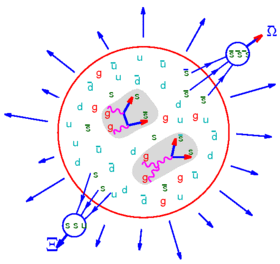
\includegraphics [width = 0.5\linewidth] {Intro/Strangeness_enhancement.png}
		\caption{Механизм образования странных кварков, основанный на модели термальной КХД.}
		\label{img:StrangenessEnhancement}  
	\end{figure}
\end{comment}
\begin{comment}
	\textbf{Динамика столкновения и уравнение состояния}
	Ожидается, что изучение коллективного движения образовавшихся адронов в конечном состоянии даст информацию о динамике столкновений тяжелых ионов. С гидродинамической точки зрения на столкновения,
	коллективное движение определяется градиентом давления сжатой ядерной материи на ранней стадии столкновения. В случае фазового перехода от порядковой ядерной к кварк-глюонной плазме ожидается соответствующее смягчение уравнения состояния за счет увеличения числа степеней свободы [4]. Таким образом, наблюдение за коллективным движением крайне важно для подтверждения гидродинамического описания динамики. Если фазовый переход первого рода, то уравнение состояния будет наиболее «мягким» при критической температуре Tc. Ожидается, что такое смягчение повлияет на динамическую эволюцию системы, поскольку внутреннее давление падает при Tc. Таким образом, наблюдение за функцией возбуждения поперечного коллективного потока может служить зондом для формирования КГП; падение функции возбуждения коллективного потока свидетельствует о пороговой энергии образования КГП.
\end{comment}

\textbf{Гашение струй.} 
Под гашением струй понимают подавление выходов адронов в области больших \pt \ ($p_T>4$ ГэВ/$c$) \cite{jet_quenching}. Высокоэнергетичные адроны образуются преимущественно в результате жестких партонных взаимодействий на начальной фазе столкновения, предшествующей образованию КГП. Таким образом, высокоэнергетичные партоны, участвовавшие в жестких рассеяниях, впоследствии взаимодействуют с кварк–глюонной средой, теряя энергию. Считается \cite{jet_quenching,InitialEnergyLoss}, что партоны теряют энергию в горячей и плотной ядерной материи вследствии глюонного тормозного излучения, что приводит к гашению струй и уменьшению \pt \ фрагментационных адронов.  Таким образом, в эксперименте наблюдается подавление выходов адронов в диапазоне $p_T > $4 ГэВ/с. 

% Cronin peak paper
%Выше $T \sim $2 ГэВ/c все большее значение приобретают процессы жесткого рассеяния. Они обеспечивают чувствительный инструмент для исследования образующейся среды. После жесткого рассеяния цветной объект (жестко рассеянный кварк или глюон) пересекает среду, образовавшуюся в результате столкновения, и сильно взаимодействует. В результате ожидается, что он потеряет энергию через индуцированное глюонное излучение. Это явление, известное как тушение струи, проявляется в виде подавления выхода адронов с высоким $p_T$ адронов, по сравнению с производством в pp-столкновениях, масштабируемым ядерной толщиной функцией $T_{AB}$, которая учитывает ядерную геометрию. Подавление измеряется в терминах фактор ядерной модификации $R_{AA} = \sigma^{AA}/T_{AB} \sigma ^{pp}$. Адронные спектры от pp-столкновений служат в качестве эталона, свободного от ядерных эффектов, и будут обсуждаться здесь в этом контексте. Важно также важно различать ядерные эффекты в начальном состоянии (холодная ядерная материя) и в конечного состояния (предположительно QGP). В RHIC столкновения d+Au при той же энергии центра масс, что и столкновения Au+Au служат этой цели. Эффект Кронина, который обычно приписывается начальному множественному рассеянию в начальном состоянии, изучается подробно.


\textbf{Ненулевые значения анизотропных коллективных потоков.}
Область перекрытия сталкивающихся релятивистских ядер имеет форму элипсоида, что приводит к возникновению градиентов давления кварк-глюонной материи. При расширении и остывании термализованной материи анизотропия давления вызывает анизотропию азимутальное импульсное распределение частиц. Количественный анализ анизотропии азимутального распределения частиц определяется посредством Фурье разложения распределения частиц по азимутальному углу $\phi$ \cite{QGP_signatures}:
$$ E \frac{d^3N}{dp^3} = \frac{1}{2\pi} \frac{d^2N}{p_T dp_T dy} 
(1+\sum_{n=1}^{N} 2v_n cos(n(\phi - \psi)))$$
где $E$ - энергия частицы;
 
$p_T$ - поперечный импульс;

$y$ - быстрота частицы;

$\phi$ - азимутальный угол частицы;
 
$\psi$ - угол плоскости реакции;

$v_n$ - коллективный поток порядка $n$. 

Величина эллиптического потока позволяет получить информацию о значениях градиентов давления при гидродинамическом расширении, эффективных степенях свободы и степени термализации системы. Зависимость эллиптического потока от размера системы, поперечного импульса или массы имеют важнейшее значение для понимания свойств материи, образующейся во время столкновений. 
В центральных столкновениях значения эллиптического потока оказываются меньше, по сравнению с перифирийными столкновениями. Это связано с тем, что в центральных столкновениях область перекрытия ядер более округлая.

\textbf{Подавление тяжелых кваркониев}
Механизм подавления следует из ожидаемой дебаевской экранировки в КГП, уменьшающей диапазон потенциалов между $c\bar{c}$  парами \cite{QGP_signatures}. Если радиус мезона больше дебаевского радиуса, определяемого соотношением температуры и плотности плазмы, мезон распадается.


\subsection{Поиски признаков образования КГП в легких системах}
Долгое время считалось, что в столкновениях легких систем, таких как столкновения $p$+Al, \heau, \dau, не достигаются условия, необходимые для образования КГП \cite{CNM, QGP_small_syst}. В связи с этим, столкновения легих систем использовались преимущественно для изучения эффектов холодной ядерной материи \cite{phi_dAu}. 
Однако в 2018 г экспериментом PHENIX были измерены ненулевые значения эллиптических и триангулярных потоков заряженных частиц в столкновениях  $p$+Au, $d$+Au, \heau \ при энергии 200 ГэВ \cite{PHENIX_Nature}. Полученные результаты были интерпретированы в рамках модели гидродинамики, предпологающей формирование КГП. С тех пор поиск эффектов КГП в легких системах столкновений является актуальной задачей физики высоких энергий. В настоящее время, помимо ненулевых значений анизотропных коллективных потоков, в столкновениях легких систем обнаружены такие признаки образования КГП как повышенный выход барионов \cite{ppg146}, эффект гашения струй \cite{pi0_smallSysts} и подавление выходов тяжелых ароматов \cite{psi_SmallSyst}. 

\textbf{Эллиптические и триангулярные потоки в $p$/$d$/\heau \ столкновениях.}
На Рисунке \ref{img:CollectivitySmallSysts} представлено сравнение значений эллиптических и триангулярных потоков $v_n(p_T)$, измеренных экспериментом PHENIX в центральных (0-5\%) a) $p$+Au b) $d$+Au и c) \heau \ столкновениях с теоретическими  предсказаниями моделей SONIC\cite{sonic}, iEBE-VISHNU\cite{iebe_vishnu} и MSTV\cite{mstv}. Данные модели используют гидродинамический подход к описанию столкновений релятивистских тяжелых ионов, что предполагает формирование КГП. 

\begin{figure}[] 
	\centerfloat
	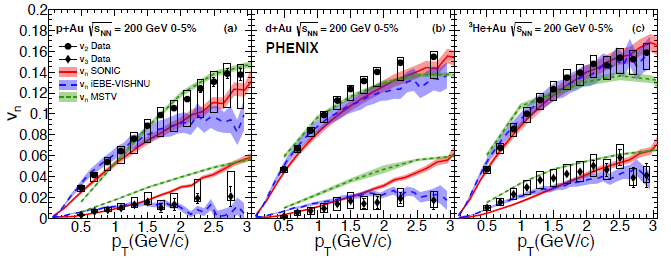
\includegraphics [width = 0.8\linewidth] {Intro/Collectivity_small_systs.png}
	\caption{Сравнение значений эллиптических и триангулярных потоков vn($p_T$), измеренных экспериментом PHENIX в центральных (0-5\%) a) $p$+Au b) $d$+Au, c) \heau \ столкновениях с теоретическими  предсказаниями моделей SONIC, iEBE-VISHNU и MSTV.}
	\label{img:CollectivitySmallSysts}   
\end{figure}


\textbf{Увеличенный выход барионов.}
Экспериментом PHENIX были измерены факторы ядерной модификации заряженных адронов (Рисунок \ref{img:CH_RAA_dAu}) и отношения выходов $p/\pi$ в столкновениях $d$+Au (Рисунок \ref{img:p2pi_dAu}) \cite{ppg146}. 
В центральных столкновениях $d$+Au наблюдается повышенный выход протонов и антипротонов, однако отношения выходов $p/\pi$ близки к значениям $p/\pi$, измеренным в $p$+$p$ столкновениях, и не проявляют статистически значимой зависимости от центральности.
Полученные результаты были интерпретированы как намек на образование КГП в столкновениях $d$+Au \cite{ppg146, PPG026}.
\begin{figure}[] 
	\centerfloat
	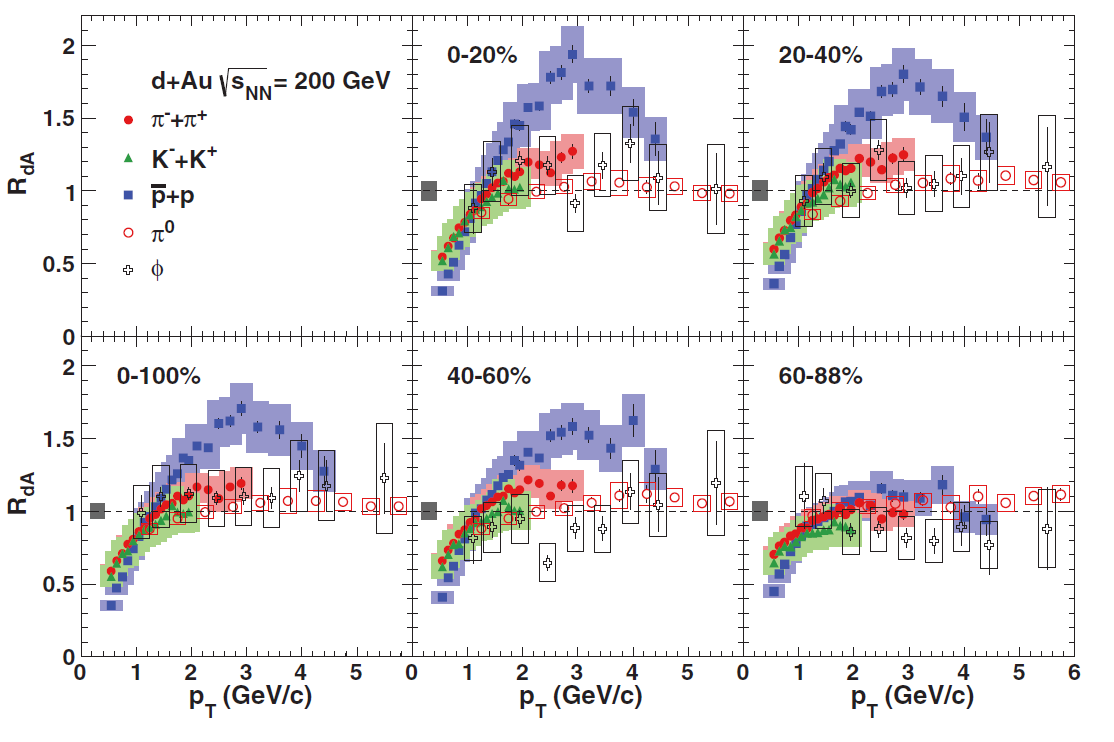
\includegraphics [width = 0.8\linewidth] {Intro/BaryonEnhancement_dAu.png}
	\caption{Факторы ядерной модификации заряженных адронов ($\pi^{+} + \pi^{-}$, $K^{+} + K^{-}$, $\bar{p}+p$, $\pi^0$, $\phi$), измеренные экспериментом PHENIX в столкновениях $d$+Au при энергии $\sqrt{s_{NN}}=$200 ГэВ.}
	\label{img:CH_RAA_dAu}   
\end{figure}

\begin{figure}[] 
	\centerfloat
	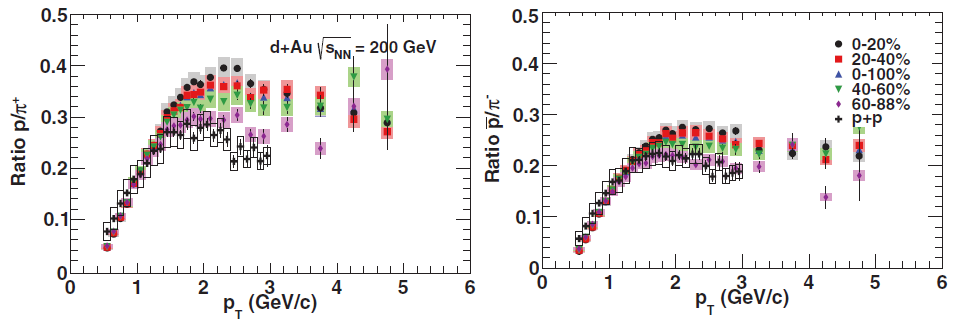
\includegraphics [width = 0.8\linewidth] {Intro/p2pi_dAu.png}
	\caption{Отношения выходов протонов к выходам $\pi^+$-мезонов ($p/\pi^{+}$) и выходов антипротонов к выходам $\pi^-$-мезонов ($\bar{p}/\pi^{-}$), измеренные экспериментом PHENIX в столкновениях $d$+Au при энергии $\sqrt{s_{NN}}=$200 ГэВ.}
	\label{img:p2pi_dAu}   
\end{figure}

\textbf{Гашение струй} % $\pi^0$ PHENIX results
Обнаружение подавления нейтральных пионов и заряженных адронов \cite{p2piRatio_130GeV, BaryonPuzzleVelkovska} в области больших $p_T$ ($p_T > 5$ ГэВ/c) в столкновениях Au+Au было одним из первых экспериментальных признаков потерь энергии партонами в сильно связанной КГП. Отсутствие подавления высокоэнергетичных адронов в столкновениях $d$+Au \cite{dAu1, dAu2}, в которых образование КГП не ожидалось, было принципиально важным для признания потерь энергии партонами в качестве признака образования КГП. Последующие систематические исследования подавления рождения высокоэнергетичных $\pi^0$ в столкновениях Au+Au при $\sqrt{s_{NN}}$ = 200 ГэВ позволили получить количественные ограничения на коэффициенты переноса среды \cite{jet_quenching_small1,jet_quenching_small2}.


\textbf{$J/\Psi$ в легких системах}
\begin{figure}[] 
	\centerfloat
	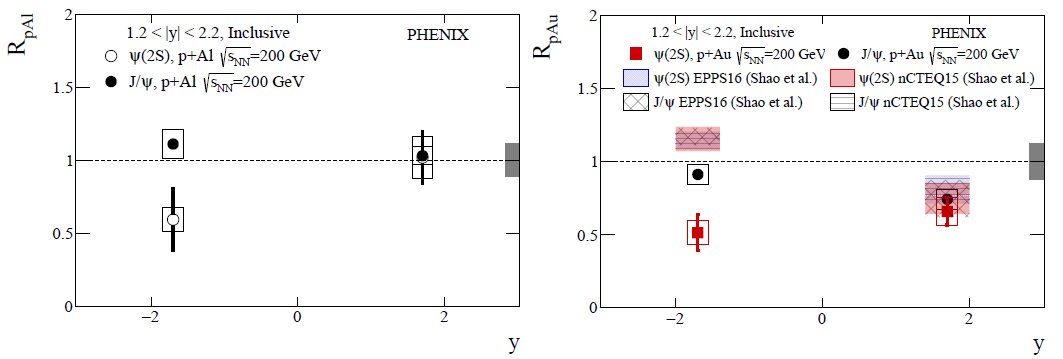
\includegraphics [width = 0.8\linewidth] {Intro/JPsi_SmallSysts}
	\caption{$J/\Psi$ в столкновениях p+Au и p+Al. }
	\label{img:JPsi_small}  
\end{figure}
Подавление состояния кваркония $\Psi(2S)$ в $d$+Au столкновениях при энергии $\sqrt{s_{NN}}=$200 ГэВ, обнаруженное экспериментом PHENIX \cite{psi_SmallSyst} также является возможным признаком эффектов нального состояния. Анализ факторов ядерной модификации $J/\Psi$ в $d$+Au столкновениях показал, что подавление выходов $J/\Psi$ в $d$+Au столкновениях могут быть описаны с помощью эффектов холодной ядерной материи.
Подавление факторов ядерной модификации $\Psi(2S)$ позднее также наблюдалось коллаборациями ALICE и LHCb в столкновениях $p$+Pb \cite{jpsi_ALICE1,jpsi_ALICE2} и были интерпретированны в рамках моделей, не учитывающих образование КГП.
Однако экспериментом PHENIX было обнаружено подавление $\Psi(2S)$-мезона, которое не согласовывалось с предсказаниями моделей, учитывающих лишь эффекты холодной ядерной материи. 


\begin{comment}
	\section{Рождение частиц в столкновениях релятивистских ионов}
	\section{Отношения частиц и химическое равновесие}
	Различия между механизмами рождения различных адронов могут быть установлены с помощью отношения их инвариантных спектров по поперечному импульсу. Установлено [], что отношения рожденных адронов хорошо описываются простой статистической моделью [].
	\begin{figure}[ht] 
		\centerfloat
		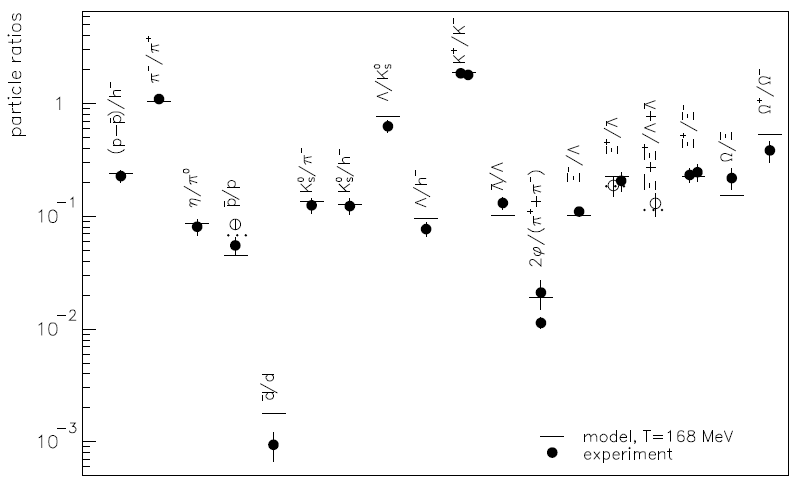
\includegraphics [width = 0.9\linewidth] {Intro/RatiosExp.png}
		\caption{Отношения выходов адронов. Сравнение между статистической моделью (горизонтальные линии) и экспериментальными отношениями (круги)} 
		\label{img:RatiosExp}  
	\end{figure}
	
	Статистическая модель основана на использовании большого канонического ансамбля для описания статистической суммы и, следовательно, плотности частиц вида $i$ в равновесном состоянии кварк-глонной материи:
	\begin{equation}
		\label{eq:Ratio}
		n_i = \frac{g_i}{2 \pi ^2}\int_0^{\infty} \frac{p^2 dp}{exp[(E_i - \mu_i)/T_{ch}]\pm 1}
	\end{equation}
	где  $n_i$ - плотность частиц, $g_i$ - спиновое вырождение, $p$ - импульс, $E$ - полная энергия и $\mu_i =\mu_B B_i - \mu_S S_i - \mu_{I_3} I_{3i}$ - химический потенциал. Величины $B_i$, $S_i$ и $I_{3i}$ представляют собой барионное число, странность и третью компоненту изоспина для частицы вида $i$. В данной модели присутствуют только два параметра: температура $T_{ch}$ и барионный химический потенциал $\mu_B$, которые являются независимыми.  На рис. ??? показано сравнение измеренных интегральных отношений выходов частиц частиц и расчетов согласно статистической модели. Как видно из рисунка, данная модель хорошо согласовывается с экспериментальными данными.
	Совпадаение экспериментальных данных с расчетсами статистической модели указывает на сохранение химического равновесия в системе. 
\end{comment}

\section{Теоретические модели}
Точное теоретическое описание процессов рождения частиц в столкновениях релятивистских тяжелых ионов невозможно в рамках квантовой хромодинамики. Это связано с непертрубативным характером некоторых процессов, таких как адронизация, а также высокой математической сложностью вычислений. В связи с этим для физической интерпретации экспериментальных результатов принято использовать различные модели, реализованные с помощью программных пакетов. Одними из наиболее широко распространенных моделей являются PYTHIA8.3 \cite{pythia} и AMPT \cite{AMPT}.

\subsection{Модель PYTHIA} \label{sec:PYTHIA}
Модель PYTHIA является программным пакетом, предназначенным для моделирования столкновений релятивистских частиц. Возможность моделирования столкновений релятивистских ионов реализована в версии PYTHIA8.3/ANGANTYR.

Согласно модели PYTHIA процесс генерации столкновения разбивается на ряд компонентов. Разделением для этих компонентов является упорядочение по времени или, что эквивалентно, по энергии и поперечному импульсу. Жесткие процессы, характеризующиеся значением $p_T > p_T^{min}$, могут быть рассчитаны в рамках пертурбативной КХД и обрабатываются в первую очередь. Мягкие и непертурбативные процессы, характеризующиеся значением $p_T < p_T^{min}$, обрабатываются в последнюю очередь, поскольку возможно только приближенное их описание. Подобное упорядочивание обработки процессов оправдано с точки зрения теоремы о факторизации, однако не является однозначным и требует корректировок на основе экспериментальных данных.

\begin{figure}[ht] 
	\center
	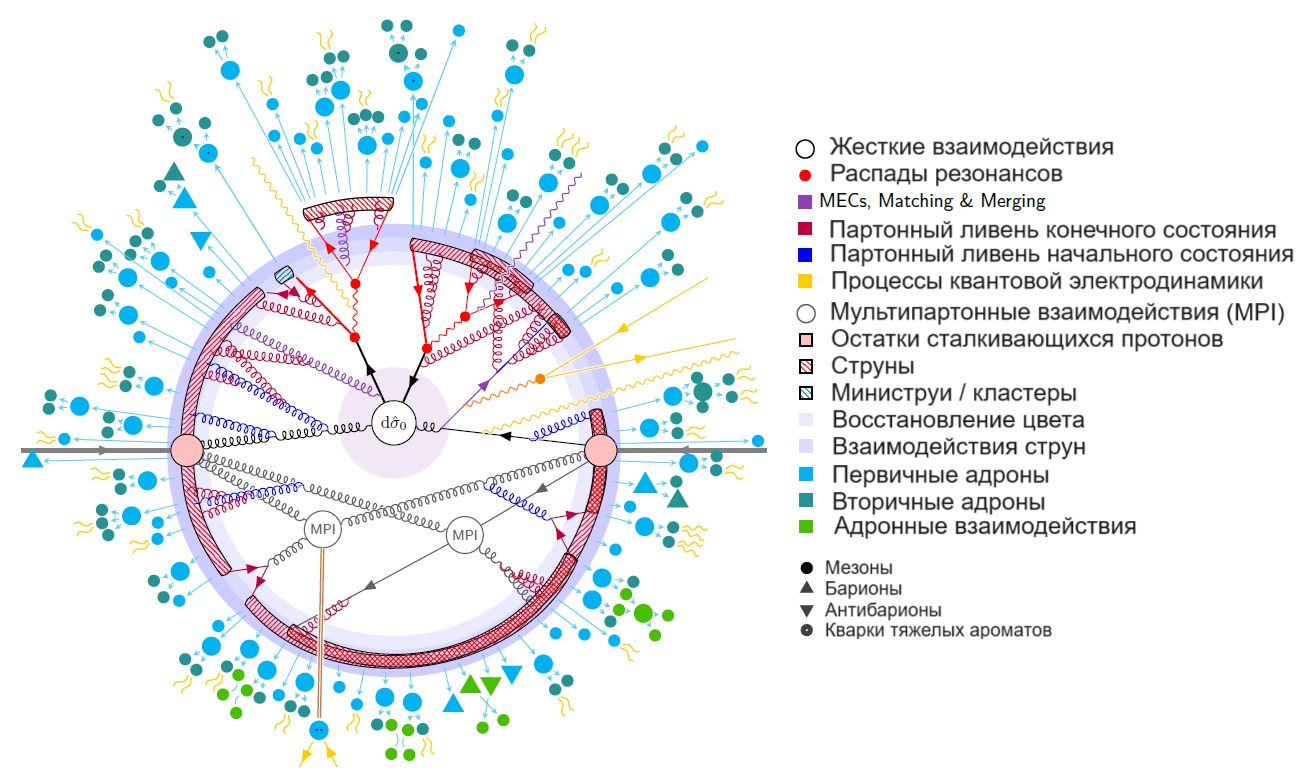
\includegraphics [width = 0.8\linewidth] {Intro/PYTHIA.png}
	\caption{Упрощенная схема моделирования $p$+$p$ столкновения в пакете PYTHIA}
	\label{img:PYTHIA}  
\end{figure}

%Упорядочивание во времени не является полностью интуитивным, по крайней мере, в направлении от прошлого к будущему. Мы скорее должны говорить о временных окнах, сосредоточенных на жестком столкновении, которые затем расширяются вперед и назад во времени, вводя последовательные явления, пока мы не останемся с парой входящих протонов, например, из пучков ускорителя, и ряд вылетающих частиц. В пространстве В пространстве импульсов мы обычно говорим о шкале "жесткости", которая характеризует каждый (суб)процесс, и часто используем меру поперечного импульса $p_T$ для его количественной оценки.

На Рисунке \ref{img:PYTHIA} приведена упрощенная схема моделирования $p$+$p$ столкновения в пакете PYTHIA.
Радиальная координата соответствует шкале по $p_T$: вблизи центра диаграммы располагаются жесткие события, а на перефирии изображены непертурбативные адронные состояния. 

Порядок моделирования $p$+$p$ столкновения является следующим:

\begin{enumerate}
	\item Рассчет жесткого рассеяния двух партонов из состава сталкивающихся адронов с помощью пертурбативной КХД. Характеристики партонов определяются с помощью партонных функций распределения.
	% Такие расчеты вводят шкалу факторизации и шкалу перенормировки. Партоны с моментами ниже этих масштабов не включаются в жесткое рассеяние, но будут введены на других этапах генерации событий. 
	
	\item Жесткий процесс может порождать набор короткоживущих резонансов, таких как $Z$ и $W^\pm$ бозоны или топ-кварки, распад которых рассматривается в тесной связи с самим жестким процессом. 
	
	\item Вычисление радиационных поправок для жесткого процесса. %фиксированного порядка могут быть включены с помощью (комбинации) матрично-элементных поправок поправок, стратегий согласования и/или слияния, см. раздел 5. На рис. 1 заштрихованная фиолетовым цветом область область вокруг жесткого процесса представляет собой диапазон масштабов, охватываемых (общей) стратегия слияния матричных элементов, активная выше некоторого заданного масштаба $p_Tmin$.
	
	\item Моделирование партонного ливня в начальном состоянии.
	
	\item Моделирование партонного ливня в конечном состоянии.
	%состоянии -  излучения в начальном состоянии.Излучение в конечном состоянии (FSR) дополнительных частиц от самого жесткого рассеяния, а также от любых резонансных распадов.
	
	\item Учет процессов рассеяния партонов, называемых многочастичными взаимодействиями. %Это явление не следует путать с "нагромождением", которое обычно относится к нескольким адрон-гадронных столкновений, зарегистрированных на одном снимке детектора.
	
	%\item Формирование струн как непертурбативного предела цветовых диполей.%На каком-то этапе после МПИ и, возможно, до резонансного распада начинают формироваться струны, как непертурбативный предел цветовых диполей. Эти диполи, однако, обычно определяются цветовыми связями, которые задаются в пределе $Nc \rightarrowtail \infty$, и не являются уникальными для Nc = 3. Как обсуждается далее в разделе 7.2, связанные с этим неоднозначности цветового пространства могут быть смоделированы с помощью цветовой пересоединенности (ЦП). Также возможно, что дальнодействующие динамические взаимодействия могут физически изменить цветовой поток и/или изменить конфигурацию расширяющихся струн перед их фрагментацией. В зависимости от характерных временных масштабов (часто которые часто не указываются явно в простых моделях КР), такие эффекты могут также называться цветовыми пересоединениями, но также могут быть отнесены к взаимодействию струн.
	
	\item Формирование синглетных по цвету подсистем, известных как струны или, в предельных случаях малой массы, как кластеры. 
	%То, что в настоящее время что осталось от входящих адронных составляющих, объединяется в остатки пучка.
	 На Рисунке \ref{img:PYTHIA} переход между партонной и адронной стадиями генерации события обозначен концентрическими окружностями, заштрихованными синим цветом.
	
	\item Образование адронов путем фрагментации струн в соответствии с Лундской струнной моделью. 
	
	\item Учет подавления Ферми-Дирака выхода идентичных частиц с полуцелым спином, близких в фазовом пространстве, или увеличения Бозе-Эйнштейна  выхода   идентичных частиц с целочисленным спином.
	
	\item Моделирование распадов нестабильных адронов, образующихся в процессе фрагментации.
	
	\item Учет адронных взаимодействий.
\end{enumerate}

Возможность моделирования столкновений релятивистских ионов реализована в модели PYTHIA8.3/ANGANTYR.
Столкновения релятивистских ионов рассматривается как экстраполяция $p$+$p$ столкновений на основе модели Глаубера. Модель PYTHIA8.3/ANGANTYR используется как одна из основных моделей для описания неколлективных эффектов.


\subsection{Модель AMPT} \label{sec:AMPT}

\begin{figure}[ht] 
	\center
	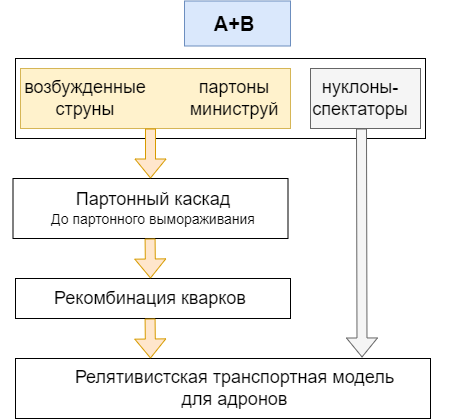
\includegraphics [width = 0.6\linewidth] {Intro/AMPT.png}
	\caption{Упрощенная схема этапов моделирования столкновения релятивистских ионов A+B согласно модели AMPTsm.}
	\label{img:AMPT}  
\end{figure}

Согласно модели AMPT процесс генерации ион-ионных столкновений разделяется на четыре основные этапа: 1) задание начальных условий, 2) расчета партонных взаимодействий, 3) моделирования перехода партонной материи в адронную, 4) расчета адронных взаимодействий. Схема генерации столкновения релятивистских ионов в модели AMPT представлена на Рисунке \ref{img:AMPT}.

\begin{enumerate}
\item Для опеределения начальных условий, включающих пространственные и импульсные распределения партонов министруй и возбуждений мягких струн, используется генератор HIJING \cite{HIJING}. HIJING является программным пакетом, основанным на методе Монте-Карло, предназначенным для изучения образования струй и связанных с ними частиц в столкновениях $p$+$p$, $p$+A и A+A высоких энергий.
 
\item Рассеяния партонов министруй и возбужденных струн моделируются с помощью партонного каскада Чжана (ZPC). В партонном каскаде рассматриваются только двучастичные рассеяния, чьи сечения вычисляются с помощью пертурбативной КХД. 

\item В версии AMPT с плавлением струн (AMPTsm) фазовый переход между партонной и адронной материи описывается с помощью рекомбинационной модели. 

\item Динамика развития адронной материи описывается адронным каскадом, который основан на транспортной модели ART, расширенной путем включения дополнительных каналов реакций, таких как образование и распад $K^*$-резонанса и антибарионных резонансов, а также рождение барионов и антибарионов из мезонов и их обратные реакции аннигиляции. 
Окончательные результаты в модели AMPT получаются после прекращения адронных взаимодействий в момент времени отсечки, после которого все наблюдаемые величины считаются неизменными.  
\end{enumerate}


\section{Мотивация}
Фазовый переход кварк-глюонной плазмы (КГП) \cite{QGP} в состояние адронного газа, называемый адронизацией КГП, является непертурбативным процессом, вследствие чего его теоретическое описание является чрезвычайно сложной задачей \cite{Coalescence_models}. В настоящее время процессы адронизации принято описывать с помощью моделей рекомбинации \cite{Coalescence_models, Recombination1, Recombination2} и моделей фрагментации \cite{FragmentationLund}. Определение параметров данных моделей осуществляется с помощью аппроксимации экспериментальных данных \cite{Coalescence_models, AMPT}. 

К основным успехам моделей рекомбинации относят описание эффекта увеличения выхода барионов в столкновениях релятивистских ионов по сравнению с $p+p$ столкновениями, считающегося признаком формирования КГП \cite{p2piRatio_130GeV, p2piRatio_2003}. Одной из измеряемых величин, с помощью которых исследуется эффект увеличенного выхода барионов, является отношение выходов протонов (антипротонов) к выходам  \pip \ (\pim) мезонов, обозначаемое как  $p/\pi^{+}$($\bar{p}/\pi^{-}$). Чем больше различие между значениями $p/\pi^{+}$($\bar{p}/\pi^{-}$), измеренными в столкновениях релятивистских ионов, и  $p/\pi^{+}$($\bar{p}/\pi^{-}$) значениями, измеренными в $p+p$ столкновениях, тем сильнее проявляется эффект увеличенного выхода барионов. 

В данной работе выполнен анализ величин $p/\pi^{+}$($\bar{p}/\pi^{-}$) в столкновениях \pal, \heau, Cu+Au при энергии \sqsn \ = 200 ГэВ и в U+U столкновениях при \sqsn \ = 193 ГэВ. Анализ экспериментальных данных был проведен путем сравнения с расчетами в рамках модели рекомбинации, реализованной в пакете AMPT \cite{AMPT}, и модели фрагментации, реализованной в пакете PYTHIA/ANGANTYR \cite{pythia}. 